%% This is an example first chapter.  You should put chapter/appendix that you
%% write into a separate file, and add a line \include{yourfilename} to
%% main.tex, where `yourfilename.tex' is the name of the chapter/appendix file.
%% You can process specific files by typing their names in at the 
%% \files=
%% prompt when you run the file main.tex through LaTeX.
\chapter{Robust MADER: Multiagent Trajectory Planner Robust to Communication Delay}\label{chap:rmader}

\section{Overviews}\label{sec:td-overviews}

Centralized trajectory planning involves a single entity controlling all agents' trajectories. This simplifies the planning process and eliminates the need for trajectory deconfliction approaches since there are no conflicts between agents. Similarly, in synchronous planning, all agents agree to execute a single set of trajectories at a synchronized point. By achieving consensus at this point, agents can obtain collision-safe trajectories and take advantage of this synchronization to resolve conflicts between their trajectories. However, these centralized and synchronous planners are limited in their scalability and are not suitable for large-scale swarms of agents.

On the other hand, in decentralized, asynchronous multiagent trajectory planning, each agent plans its own trajectory, and agents communicate and exchange their trajectories asynchronously. Therefore, a trajectory deconfliction scheme is critical for ensuring collision-free trajectories among agents. The deconfliction scheme utilizes the trajectories shared between agents and resolves conflicts in an asynchronous manner, allowing for scalable and robust trajectory planning in large-scale swarms. 

\section{Trajectory Deconfliction}

\subsection{MADER's trajectory deconfliction}

MADER~\cite{tordesillas2020mader} is among the first fully decentralized and asynchronous trajectory planners that guarantee collision-free trajectories under ideal communication through the use of the planning stages shown in Fig.~\ref{fig:mader_deconfliction}. As described in Section~\ref{sec:literature_review}, existing methods, including MADER, either implicitly or explicitly assume perfect communication environments, and with the presence of communication latency, their approaches' collision-safety guarantee no longer holds.

For instance, in MADER, an agent plans its initial trajectory during \OptimizationStep{} (\OStep{}), followed by \CheckStep{} (\CStep{}) to ensure its plan does not lead to a collision.
Finally, \RecheckStep{} (\RStep{}) is used to check if the agent received any trajectory updates from other agents during \CStep{} - if so, an agent starts over planning at \OStep{}.
Although MADER does not have explicit safety guarantees in the presence of communication delays, its trajectories are still collision-free for cases 1 and 2 shown in Fig.~\ref{fig:mader_deconfliction}. However,  collisions may occur in cases 3 and 4 of Fig.~\ref{fig:mader_deconfliction}.
These four cases are summarized in Fig.~\ref{fig:mader_deconfliction} and Table~\ref{tab:safety_guarantees_delays}.

\begin{figure*}[t]
\centering
  \centering
  \resizebox{1.0\textwidth}{!}{%
    \begin{tikzpicture}
        [
        % define styles
        greenbox/.style={shape=rectangle, fill=opt_color, draw=black},
        bluebox/.style={shape=rectangle, fill=check_color, draw=black},
        redbox/.style={shape=rectangle, fill=recheck_color, draw=black},
        ]
        
        % coordinate
        \newcommand\Ay{5.5}
        \newcommand\Axo{3}
        \newcommand\Axc{8}
        \newcommand\Axr{10}
        \newcommand\Axe{11}
        
        \newcommand\By{2}
        \newcommand\Bxo{5}
        \newcommand\Bxc{12}
        \newcommand\Bxr{15}
        
        % MADER deconfliction 
        % Agent A
            \node[text=red] at (0.5,\Ay+0.2) {\scriptsize Agent A};
            % previous iter.
            \filldraw[fill=check_color, draw=black, opacity=0.2] (0,\Ay) rectangle (1.5,\Ay-1.0);
            \filldraw[fill=recheck_color, draw=black, opacity=0.2] (1.5,\Ay) rectangle (\Axo,\Ay-1.0);
            % current iter.
            \filldraw[thick, fill=opt_color, draw=black] (\Axo,\Ay) rectangle (\Axc,\Ay-1.0);
            \filldraw[thick, fill=check_color, draw=black] (\Axc, \Ay) rectangle (\Axr, \Ay-1.0);
            \filldraw[thick, fill=recheck_color, draw=black] (\Axr, \Ay) rectangle (\Axe, \Ay-1.0);
            % next iter.
            \filldraw[fill=opt_color, draw=black, opacity=0.2] (\Axe, \Ay) rectangle (\Axe+4.5, \Ay-1.0);
            \filldraw[fill=check_color, draw=black, opacity=0.2] (\Axe+4.5, \Ay) rectangle (\Axe+5.5, \Ay-1.0);
            \filldraw[fill=recheck_color, draw=black, opacity=0.2] (\Axe+5.5, \Ay) rectangle (\columnwidth, \Ay-1.0);
        % Agent B
            \node[text=blue] at (0.5,\By+0.2) {\scriptsize Agent B};
            % previous iter.
            \filldraw[fill=check_color, draw=black, opacity=0.2] (0,\By) rectangle (\Bxo-0.5,\By-1.0);
            \filldraw[fill=recheck_color, draw=black, opacity=0.2] (\Bxo-0.5,\By) rectangle (\Bxo,\By-1.0);
            % current iter.
            \filldraw[thick, fill=opt_color, draw=black] (\Bxo,\By) rectangle (\Bxc,\By-1.0);
            \filldraw[thick, fill=check_color, draw=black] (\Bxc, \By) rectangle (\Bxr, \By-1.0);
            \filldraw[thick, fill=recheck_color, draw=black] (\Bxr, \By) rectangle (\Bxr+1, \By-1.0);
            % next iter.
            \filldraw[fill=opt_color, draw=black, opacity=0.2] (\Bxr+1, \By) rectangle (\columnwidth, \By-1.0);

        \draw[thick, densely dotted] (\Axe,-0.0) -- (\Axe,\Ay-1.0) node[] at (\Axe, -0.3) {\tiny $t_{\trajA{}{}}^A$};
            
        % Axis
        \draw[thick,->] (0,0) -- (\columnwidth,0) node[anchor=north east] {time};
        
        % traj. msgs
        \draw[thick, ->, draw=red] (\Axe,\Ay-1.0) -- (\Axe,\Ay-2.2) node[midway,fill=white, text=red] {\tiny \trajA{}};
        \draw[thick, <-, draw=red] (\Bxc-0.3,\By) -- (\Bxc-0.3,\By+0.3) node[anchor=south,text=black] {\tiny case 1};
        \draw[thick, <-, draw=red] (\Bxc+0.5,\By) -- (\Bxc+0.5,\By+0.3) node[anchor=south,text=black] {\tiny case 2};
        \draw[thick, <-, draw=red] (\Bxr+0.1,\By) -- (\Bxr+0.1,\By+0.3) node[anchor=south,text=black] {\tiny case 3};
        \draw[thick, <-, draw=red] (\Bxr+2,\By) -- (\Bxr+2,\By+0.3) node[anchor=south,text=black] {\tiny case 4};
        
        % legend in the sequence
        \node[font=\bfseries,right] at (\Axo,\Ay-0.15) {\tiny Optimization (O\textsubscript{A})};
        \node[font=\bfseries,right] at (\Axc,\Ay-0.15) {\tiny Check (C\textsubscript{A})};
        \node[font=\bfseries,right] at (\Axr-0.47,\Ay+0.15) {\tiny Recheck (R\textsubscript{A})};

        \node[font=\bfseries,right] at (\Bxo,\By-0.15) {\tiny O\textsubscript{B}};
        \node[font=\bfseries,right] at (\Bxc,\By-0.15) {\tiny C\textsubscript{B}};
        \node[font=\bfseries,right] at (\Bxr,\By-0.15) {\tiny R\textsubscript{B}};
        
        % text
        \node[color=gray] at (1.0,\Ay-0.15) {\scriptsize Prev. iter.};
        \node[color=gray] at (0.95\columnwidth,\Ay-0.15) {\scriptsize Next iter.};
        \node[color=gray] at (1,\By-0.15) {\scriptsize Prev. iter.};
        \node[color=gray] at (0.95\columnwidth,\By-0.15) {\scriptsize Next iter.};
    \end{tikzpicture}
    }
    \caption[MADER trajectory deconfliction]{MADER deconfliction: \AgentA{} solves \OStepA{} to find its optimal trajectory, constrained by other agents' trajectories. \AgentA{} then begins \CStepA{} to determine if that generated trajectory has any conflicts with trajectories received during \OStepA{}. Finally, in \RStepA{}, \AgentA{} checks if it received any trajectories during \CStep{}. The four cases shown in the figure correspond to different communication delays, resulting in \trajA{} being received by \AgentB{} at different times. Designed to guarantee safety when there are no communication delays, MADER also guarantees safety when \trajA{} arrives during \OStepB{} (Case 1) or \CStepB{} (Case 2), but could cause collisions if \trajA{} is received during/after (Case 3/4) \RStepB{}.}
  \label{fig:mader_deconfliction}
\end{figure*}

\subsection{RMADER's trajectory deconfliction}

To achieve robustness to communication delays, we replace the \RecheckStep{} with \DelayCheckStep{} (\DCStep{}), where each agent repeatedly checks if its newly optimized trajectory conflicts with other agents' trajectories.
If an agent detects conflicts during \DCStep{}, it discards the new trajectory and starts another \OStep{} while executing its previous trajectory. 
If no collisions are detected in \DCStep{}, it starts executing the new trajectory. 
To guarantee collision-free trajectory generation, \DCStep{} needs to be longer than the possible longest communication delay (i.e., \NeccessaryCond{}). 
That way, an agent can always keep at least one collision-free trajectory. 
It could, however, not be ideal for introducing such a long \delayParameter{}, and therefore, in Chapter~\ref{chap:simulation-results} we also tried $\delta_{\text{DC}}<\delta_{\text{max}}$ and measure its performance. 
Fig.~\ref{fig:rmader_deconfliction} shows how RMADER deals with communication delays.
Furthermore, Table~\ref{tab:safety_guarantees_delays} shows all the possible cases in which communication delays could occur and how these are handled by RMADER to generate collision-free trajectories even with communication delays.
The pseudocode of RMADER deconfliction is given in Algorithm~\ref{alg:rmader}. First, Agent~B runs \OStep{} to obtain \trajBNew{} and broadcasts it if \CStep{} is satisfied 
(Line~\ref{line:broadcast_traj_B_new}). This \CStep{} aims to determine if \trajBNew{} has any conflicts with trajectories received in \OStep{}. Then, Agent~B commits either \trajBPrev{} or \trajBNew{} - if \DCStep{} detects conflicts, Agent~B commits to \trajBPrev{} (Line~\ref{line:DC_not_satisfied}), and if \DCStep{} detects no conflicts, \trajBNew{} (Line~\ref{line:DC_satisfied}). This committed trajectory is then broadcast to the other agents (Line~\ref{line:broadcast_traj_B}). Table~\ref{tab:mader_vs_rmader} highlights the differences between MADER and RMADER.

\begin{figure*}[t]
\centering
  \resizebox{1.0\textwidth}{!}{%
       \begin{tikzpicture}
       [
        % define styles
        greenbox/.style={shape=rectangle, fill=opt_color, draw=black},
        bluebox/.style={shape=rectangle, fill=check_color, draw=black},
         yellowbox/.style={shape=rectangle, fill=delaycheck_color, draw=black},
        ]
        
        % coordinate
        \newcommand\Ay{5.5}
        \newcommand\Axo{3}
        \newcommand\Axc{8}
        \newcommand\Axr{10}
        \newcommand\Axe{11}
        
        \newcommand\By{2}
        \newcommand\Bxo{5}
        \newcommand\Bxc{12}
        \newcommand\Bxr{15}
        \newcommand\Bxe{17}
        
        % RMADER deconfliction 
        % Agent A
            \node[text=red] at (0.5,\Ay+0.2) {\scriptsize Agent A};
            % previous iter.
            \filldraw[fill=check_color, draw=black, opacity=0.2] (0,\Ay) rectangle (1.5,\Ay-1.0);
            \filldraw[fill=delaycheck_color, draw=black, opacity=0.2] (0.5,\Ay) rectangle (\Axo,\Ay-1.0);
            % current iter.
            \filldraw[thick, fill=opt_color, draw=black] (\Axo,\Ay) rectangle (\Axc,\Ay-1.0);
            \filldraw[thick, fill=check_color, draw=black] (\Axc, \Ay) rectangle (\Axr, \Ay-1.0);
            \filldraw[thick, fill=delaycheck_color, draw=black] (\Axr, \Ay) rectangle (\Axe, \Ay-1.0);
            % next iter.
            \filldraw[fill=opt_color, draw=black, opacity=0.2] (\Axe, \Ay) rectangle (\Axe+1.5, \Ay-1.0);
            \filldraw[fill=check_color, draw=black, opacity=0.2] (\Axe+1.5, \Ay) rectangle (\columnwidth, \Ay-1.0);
        % Agent B
            \node[text=blue] at (0.5,\By+0.2) {\scriptsize Agent B};
            % previous iter.
            \filldraw[fill=check_color, draw=black, opacity=0.2] (0,\By) rectangle (\Bxo-0.5,\By-1.0);
            \filldraw[fill=delaycheck_color, draw=black, opacity=0.2] (\Bxo-0.5,\By) rectangle (\Bxo,\By-1.0);
            % current iter.
            \filldraw[thick, fill=opt_color, draw=black] (\Bxo,\By) rectangle (\Bxc,\By-1.0);
            \filldraw[thick, fill=check_color, draw=black] (\Bxc, \By) rectangle (\Bxr, \By-1.0);
            \filldraw[thick, fill=delaycheck_color, draw=black] (\Bxr, \By) rectangle (\Bxe, \By-1.0);
            % next iter.
            \filldraw[fill=opt_color, draw=black, opacity=0.2] (\Bxe, \By) rectangle (\columnwidth, \By-1.0);
            % \filldraw[fill=check_color, draw=black, opacity=0.2] (\Bxe+1.0, \By) rectangle (\columnwidth-1, \By-1.0);
        
        % time label
        % \draw[thick, densely dotted] (\Axo,0) -- (\Axo,\Ay-1.0) node[] at (\Axo, -0.25) {\tiny $t_o^A$};
        %\draw[thick, densely dotted] (\Axc,0) -- (\Axc,\Ay-1.0) node[] at (\Axc, -0.25) {\tiny $t_c^A$};
        \draw[thick, densely dotted] (\Axr,0) -- (\Axr,\Ay-1.0) node[] at (\Axr, -0.25) {\tiny t\textsubscript{traj\textsubscript{A\textsubscript{new}}}};
        \draw[thick, densely dotted] (\Axe,0) -- (\Axe,\Ay-1.0) node[] at (\Axe, -0.25) {\tiny t\textsubscript{traj\textsubscript{A}}};
            
        % Axis
        \draw[thick,->] (0,0) -- (\columnwidth,0) node[anchor=north east] {time};
        
        % traj. msgs
        \draw[thick, ->, draw=red] (\Axr,\Ay-1.0) -- (\Axr,\Ay-2.2) node[midway,fill=white, text=red] {\tiny \trajANew{}};
        \draw[thick, ->, draw=red] (\Axe,\Ay-1.0) -- (\Axe,\Ay-2.2) node[midway,fill=white, text=red] {\tiny \trajA{}};
        \draw[thick, <-, draw=red] (\Bxc-0.2,\By) -- (\Bxc-0.2,\By+0.3)  node[anchor=south,text=black] {\tiny case 1};
        \draw[thick, <-, draw=red] (\Bxc+0.6,\By) -- (\Bxc+0.6,\By+0.3) node[anchor=south,text=black] {\tiny case 2};
        \draw[thick, <-, draw=red] (\Bxr+0.4,\By) -- (\Bxr+0.4,\By+0.3) node[anchor=south,text=black] {\tiny case 3};
        \draw[thick, <-, draw=red] (\Bxe+0.4,\By) -- (\Bxe+0.4,\By+0.3) node[anchor=south,text=black] {\tiny case 4};
        
        % legend in the sequence
        \node[font=\bfseries,right] at (\Axo,\Ay-0.15) {\tiny O\textsubscript{A}};
        \node[font=\bfseries,right] at (\Axc,\Ay-0.15) {\tiny C\textsubscript{A}};
        \node[font=\bfseries,right] at (\Axr,\Ay-0.15) {\tiny DC\textsubscript{A}};

        \node[font=\bfseries,right] at (\Bxo,\By-0.15) {\tiny O\textsubscript{B}};
        \node[font=\bfseries,right] at (\Bxc,\By-0.15) {\tiny C\textsubscript{B}};
        \node[font=\bfseries,right] at (\Bxr,\By-0.15) {\tiny DC\textsubscript{B}};
        
        % legend box
        % \matrix [draw,below left] at (current bounding box.north east) {
        % \matrix [draw,below left,fill=white,opacity=1.0] at (15, \Ay) {
        %   \node [greenbox,label=right:Optimization] {}; \\
        %   \node [bluebox,label=right:Check] {}; \\
        %   \node [redbox,label=right:Recheck] {}; \\
        % };
        
        % text
        \node[color=gray] at (1,\Ay-0.15) {\scriptsize Prev. iter.};
        \node[color=gray] at (0.95\columnwidth,\Ay-0.15) {\scriptsize Next iter.};
        \node[color=gray] at (1,\By-0.15) {\scriptsize Prev. iter.};
        \node[color=gray] at (\columnwidth,\By-1.45) {\scriptsize Next iter.};
        
    \end{tikzpicture}
    }
    
  \caption[RMADER trajectory deconfliction]{RMADER deconfliction: After \CStepA{}, \AgentA{} keeps executing the trajectory from the previous iteration, \trajAPrev{}, while checking potential collisions of newly optimized trajectory, \trajANew{}. 
  This is because \trajANew{} might have conflicts due to communication delays and need to be checked in \DCStepA{}, and traj\textsubscript{A\textsubscript{prev}} is ensured to be collision-free. If collisions are detected in either \CStepA{} or \DCStepA{}, \AgentA{} keeps executing \trajAPrev{} (i.e., $\text{\trajA{}}\leftarrow \text{\trajAPrev{}}$). If \DCStepA{} does not detect collisions, \AgentA{} broadcasts and starts implementing \trajANew{} (i.e., $\text{\trajA{}}\leftarrow \text{\trajANew{}}$).}
  \label{fig:rmader_deconfliction}
\end{figure*}

\begin{table}[b]
    \begin{centering}
    \caption[Definitions of communication delay quantities]{Definitions of the different delay quantities: Note that, by definition, $0\le\delayIntroduced\le\delayActual{}\le\delayActualMax{}$. See also Fig~\ref{fig:comm_delay_on_mesh_centr} for the actual histogram of the delays in simulation and hardware, respectively.}
    \renewcommand{\arraystretch}{2}
    \begin{centering}
    \begin{tabular}{>{\centering\arraybackslash}m{0.1\columnwidth} >{\arraybackslash}m{0.7\columnwidth}}
    \toprule 
    \delayActual{} & Actual communication delays among agents. \tabularnewline
    \hline 
    \delayActualMax{} & \makecell[l]{Possible maximum communication delay. } \tabularnewline
    \hline 
    \delayIntroduced{} & \makecell[l]{Introduced communication delay in simulations. } \tabularnewline
    \hline 
    \delayParameter{} & \makecell[l]{Length of \DelayCheckStep{} in RMADER. \\ To guarantee safety, $\delayActualMax{}\le\delayParameter{}$ must be satisfied.} \tabularnewline
    \bottomrule
    \end{tabular}
    \par\end{centering}
    \label{tab:delaydefinitions}
    \par\end{centering}
\end{table}

\begin{algorithm}[h]
    \begin{algorithmic}[1]
    \Require traj\textsubscript{B}, a feasible trajectory
    \While{not goal reached}
        \State \trajBNew{} $=$ \textproc{\OptimizationStep{}()} \label{line:traj_opt}
        \If{\textproc{\CheckStep}(\trajBNew{}) $==$ False} 
            \State Go to Line 2
        \EndIf
        \State Broadcast \trajBNew{} \label{line:broadcast_traj_B_new}
        \If{\textproc{\DelayCheckStep{}}(\trajBNew{}) $==$ False} 
            \State \trajB{} $\leftarrow$ \trajBPrev{}, and go to Line~\ref{line:broadcast_traj_B}\label{line:DC_not_satisfied}
        \EndIf
        \State \trajB{} $\leftarrow$ \trajBNew{} \label{line:DC_satisfied}
        \State Broadcast \trajB{} \label{line:broadcast_traj_B}
    \EndWhile
    \end{algorithmic}
    \caption{Robust MADER - Agent B}
    \label{alg:rmader}
\end{algorithm}

\begin{algorithm}[h]
    \newcommand{\algorithmicbreak}{\textbf{break}}
    \begin{algorithmic}[1] %1 means every 1 line the line will be numbered
    \Function {\textproc{\DelayCheckStep{}}}{\trajBNew{}}
        \For {\delayParameter{} seconds}
            \If{\trajBNew{} collides with any trajectory in $\mathcal{Q}_B$}    
                %\State Discards \trajB{}
                \State \Return False
             \EndIf
         \EndFor
    \State \Return True
    \EndFunction
    \end{algorithmic}
    \caption{Delay Check - Agent B}\label{alg:pess_delaycheck}
\end{algorithm}

\begin{table}
\caption[MADER and RMADER's safety guarantees under communication delays]{Safety guarantees under communication delays: Depending on when \trajA{} is received by Agent B, the deconfliction takes place at different stages. MADER does not guarantee safety if \trajA{} is received during \RStepB{} or during the following iteration, while RMADER guarantees safety in all the cases. Note that in RMADER, if Agent~B does not receive \trajA{} by the end of \DCStepB{}, then the deconfliction is performed by Agent A (specifically, in \CStepA{} or \DCStepA{}) and not by Agent B. Agent A will use \trajBNew{} and/or \trajB{} for this.}
\label{tab:safety_guarantees_delays}
\begin{centering}
\renewcommand{\arraystretch}{1.2}
\resizebox{1.0\columnwidth}{!}{
\setlength\extrarowheight{0.3em}
\begin{tabular}{>{\centering}m{0.3\columnwidth} || >{\centering}m{0.2\columnwidth} >{\centering}m{0.2\columnwidth} >{\centering}m{0.2\columnwidth} >{\centering}m{0.2\columnwidth}}
\toprule
\multicolumn{1}{>{\centering}m{0.1\columnwidth}||}{} & \multicolumn{4}{c}{\textbf{MADER}} \tabularnewline[0.2em]
\hline
\textbf{When \trajA{} received}  & \makecell{\OStepB{} \\ (Case 1)} & \makecell{\CStepB{} \\ (Case 2)} & \makecell{\RStepB{} \\ (Case 3)} & \makecell{\textbf{Next iter.} \\ (Case 4)} \tabularnewline[0.4em]
\hline 
\textbf{\trajA{} deconflicted? When?} & \makecell{\YesGreen{} \\ \CStepB{}}  & \makecell{\YesGreen{} \\ \RStepB{}}  & \NoRed{}  & \NoRed{} \tabularnewline
\bottomrule
\end{tabular}
}

\resizebox{1.0\columnwidth}{!}{
\setlength\extrarowheight{0.3em}
\begin{tabular}{>{\centering}m{0.3\columnwidth} || >{\centering}m{0.2\columnwidth} >{\centering}m{0.2\columnwidth} >{\centering}m{0.2\columnwidth} >{\centering}m{0.2\columnwidth}}
\toprule
\multicolumn{1}{>{\centering}m{0.1\columnwidth}||}{} & \multicolumn{4}{c}{\textbf{RMADER}}\tabularnewline
\hline
\textbf{When \trajANew{}/\trajA{} received}  & \makecell{\OStepB{} \\ (Case 1)} & \makecell{\CStepB{} \\ (Case 2)} & \makecell{\DCStepB{} \\ (Case 3)} & \makecell{\textbf{Next iter.} \\ (Case 4)} \tabularnewline
\hline 
\textbf{\trajANew{}/\trajA{} deconflicted? When?} & \makecell{\YesGreen{} \\ \CStepB{}} & \makecell{\YesGreen{} \\ \DCStepB{}}  & \makecell{\YesGreen{} \\ \DCStepB{}}  & \makecell{\YesGreen{} \\ \CStepA{} or \DCStepA{}} \tabularnewline
\bottomrule
\end{tabular}
}
\par\end{centering}
\end{table}

\begin{table}[h]
\begin{centering}
\caption{\centering Differences between MADER and RMADER}
\label{tab:mader_vs_rmader}
\renewcommand{\arraystretch}{1.1}
\resizebox{1.0\columnwidth}{!}{
\scriptsize
\begin{tabular}{>{\centering\arraybackslash}m{0.4\columnwidth} >{\centering\arraybackslash}m{0.4\columnwidth}}
\toprule
\textbf{MADER} & \textbf{RMADER}\tabularnewline
\hline 
\hline 
Upon successful \CStep{} and \RStep{}, the newly optimized trajectory is broadcast to other agents 
%Broadcast only the committed trajectory. This committed trajectory will be newly optimized trajectory if both \CStep{} and \RStep{} are satisfied, and the previous trajectory
& Upon successful \CStep{}, \trajJNew{} is broadcast. After \DCStep{}, the committed trajectory \trajJ{} (which is either \trajJNew{} and \trajJPrev{} depending on whether \DCStep{} is satisfied or not) is broadcast \tabularnewline
\hline 
\RStep{} is a Boolean check to see if the agent received traj.
in \CStep{} & \DCStep{} is a sequence of collision checks\tabularnewline
\hline 
\RStep{} is very short & \DCStep{} lasts \delayParameter{} seconds\tabularnewline
\bottomrule
\end{tabular}
}
\par\end{centering}
\end{table}

\newcommand{\QB}{\ensuremath{\mathcal{Q}_B}}

Agent~B stores the trajectories received from other agents in a set \QB{}; for example, for each Agent~J, Agent~B will store the committed trajectory of Agent~J, \trajJ{}, and possibly the newly optimized trajectory \trajJNew{} if any new committed trajectory has still not been broadcast. Figure~\ref{fig:QB_definition} shows the way Agent B stores trajectories from Agent A. 
\QB{} is used in \OStep{}, \CheckStep{}, and \DCStep{},  where Agent~B checks for collision against all the trajectories stored in \QB{}. Note that \QB{} is updated in parallel with \OStep{} and \DCStep{}. 
At the beginning of \OStepB{}, an agent generates an optimal trajectory, \trajBNew{}, using all the trajectories stored in \QB{} as constraints, and then, Agent B checks for \trajBNew{}'s potential collisions against \QB{}, which is updated in optimization. 
Finally, Agent~B repeatedly checks for collisions against \QB{} in \DCStepB{}, which lasts for \delayParameter{}. 
Note that \CStep{} is not necessary to guarantee safety in RMADER - \OStep{} followed by \DCStep{} alone can generate collision-free trajectories as long as \NeccessaryCond{} holds. Though \CStep{} detects collisions before broadcasting any (possibly conflicted) trajectories and allows an agent to start another \OStep{}, which prevents unnecessary communication.

\begin{figure}[h]
    \centering
    \includegraphics[width=0.6\columnwidth]{figures/QB_definition.pdf}
    \setlength{\belowcaptionskip}{-0.5em}
    \caption[Trajectory storing scheme]{Agent~B stores in \QB{} the last committed trajectory of Agent~A. It will also contain the newly optimized trajectory \trajANew{} while the new committed trajectory has still not been received by Agent~B. }
    \label{fig:QB_definition}
\end{figure}

Now we provide a theoretical analysis of RMADER's trajectory deconfliction. 
First, we introduce Lemma~\ref{lem:two_agent_suffices_multiagent}, which allows us to scale up and apply two-agent deconfliction analysis to multiagent deconfliction, and then Proposition~\ref{prop:rmader_deconfliction_theorem} provides a theoretical guarantee of RMADER's deconfliction approach. 

\newtheorem{lemma}{Lemma}
\begin{lemma}
\label{lem:two_agent_suffices_multiagent}
In decentralized asynchronous trajectory planning, collision safety guarantee between any two agents is a sufficient condition for multiagent collision safety guarantee. 
\end{lemma}

\begin{proof}
Decentralized asynchronous multiagent trajectory deconfliction is a set of two-agent trajectory deconfliction, and therefore in case of trajectory deconfliction is guaranteed between every pair of any two agents, multiagent trajectory deconfliction is also guaranteed. 
\end{proof}

\newtheorem{prop}{Proposition}
\begin{prop}
\label{prop:rmader_deconfliction_theorem}
Given $\delayParameter{}>\delayActualMax{}$, RMADER is guaranteed to be collision-free under communication delay.
\end{prop}

\begin{proof}
By Lemma~\ref{lem:two_agent_suffices_multiagent}, to prove RMADER's multiagent collision-free guarantee, we show RMADER's collision-free guarantee between two agents.
Note that in case the decentralized asynchronous planner uses hard constraints, such as RMADER, as long as at any given time, at least one of the two agents has knowledge of the other agent's trajectory, collision safety is guaranteed between the two agents \textemdash In RMADER, this condition is implied by $\delayParameter{}>\delayActualMax{}$. 
To prove RMADER's collision-free guarantee, we thoroughly go through all the possible 12 cases of trajectory deconfliction between two agents - One agent sends its trajectory to the other agent's either \OStep{}, \CStep{}, or \DCStep{}, and the other agent can receive this trajectory in either \OStep{}, \CStep{}, \DCStep{}, or the next iteration. 
For clarity, we define the time \AgentA{} publishes its newly optimized trajectory as \tApub, the time \AgentB{} receives it as \tBrec, and Agent B's \OptimizationStep/\CheckStep/\DelayCheckStep{} as \OStepB/\CStepB/\DCStepB, respectively. All the possible cases are illustrated in Table~\ref{tab:rmader_possible_cases}; for example, case 3 denotes \AgentA{} publishes in \OStepB{}, and \AgentB{} receives it in \DCStepB{}. Note that cases 1-4 correspond to cases 1-4 in Fig.~\ref{fig:rmader_deconfliction}.

\begin{table}[h]
\caption{\centering RMADER Trajectory Deconfliction Cases}
\label{tab:rmader_possible_cases}
\begin{centering}
\renewcommand{\arraystretch}{1.0}
\resizebox{0.7\columnwidth}{!}{
\begin{tabular}{ c c || c c c c }
\toprule
 & & \multicolumn{4}{c}{\tBrec}\tabularnewline
\cline{3-6} 
 & & \OStepB{} & \CStepB{} & \DCStepB{} & Next Iter. \tabularnewline
\hline \hline
\multirow{3}[1]{*}{\tApub} & \OStepB{} & case 1 & case 2 & case 3 & case 4 \tabularnewline
\cline{2-6} 
 & \CStepB{} & case 5 & case 6 & case 7 & case 8 \tabularnewline
\cline{2-6}
 & \DCStepB{} & case 9 & case 10 & case 11 & case 12 \tabularnewline
\bottomrule
\end{tabular}}
\par\end{centering}
\end{table}

\begin{itemize}
\item In Case 1, Agent B detects possible collisions in its \CStep{} before committing to any trajectory.
\item In Case 2, Agent B detects possible collisions in its \DCStep{} before committing to any trajectory.
\item In Case 3, Agent B detects possible collisions in its \DCStep{} before committing to any trajectory.
\item In Case 4, Given $\delayParameter{}>\delayActualMax{}$, this case will never occur.
\item Case 5 will never occur since \CStep{} comes after \OStep{}.
\item In Case 6, Agent B detects possible collisions in its \DCStep{} before committing to any trajectory.
\item In Case 7, Agent B detects possible collisions in its \DCStep{} before committing to any trajectory.
\item Case 8 will never occur because $\delayParameter{}>\delayActualMax{}$.
\item Case 9 will never occur since \DCStep{} comes after \OStep{}.
\item Case 10 will never occur since \DCStep{} comes after \CStep{}.
\item In Case 11, Agent B detects possible collisions in its \DCStep{} before committing to any trajectory.
\item In Case 12, Agent B will commit its trajectory at the end of its \DCStep{}, not knowing Agent A's potentially collision-prone trajectory. However, by $\delayParameter{}>\delayActualMax{}$, Agent B's newly optimized trajectory is published in either Agent A's \OStep{} or \CStep{}, and therefore, Agent A can detect potential collisions before committing to its trajectory.
\end{itemize}

As shown above, in all the possible cases, either one of the two can detect possible collisions. Therefore RMADER is guaranteed to be collision-free as long as $\delayParameter{}>\delayActualMax{}$ holds.
\end{proof}

\subsection{RMADER without Check}

As demonstrated in Algorithm~\ref{alg:pess_delaycheck}, \DCStep{} repeatedly executes \CheckStep{}, and therefore we can guarantee safety without \CheckStep{} as long as \DCStep{} is longer than \delayActualMax{}. However, this could increase the number of rejections of newly optimized trajectory because it is published before it is checked for potential collisions with trajectories received in \OStep, leading to more conservative results.
Note that even if we skip \CheckStep{} and publish \trajNew{}, \trajNew{} is not committed yet, and therefore, collision-free guarantee is ensured. Fig.~\ref{fig:wo_check_rmader_deconfliction} illustrates this scheme's trajectory deconfliction: 
\begin{itemize}
    \item Case 1 \& 2: \AgentB{} can detect its trajectory conflicts in \DCStepB.
    \item Case 3: As long as $\delayParameter{}>\delayActualMax{}$, Case 3 will not happen.
\end{itemize}

\begin{figure}[h]
\centering
  \centering
  \resizebox{1.0\textwidth}{!}{%
       \begin{tikzpicture}
       [
        % define styles
        greenbox/.style={shape=rectangle, fill=opt_color, draw=black},
        bluebox/.style={shape=rectangle, fill=check_color, draw=black},
         yellowbox/.style={shape=rectangle, fill=delaycheck_color, draw=black},
        ]
        
        % coordinate
        % coordinate
        \newcommand\Ay{5.5}
        \newcommand\Axo{3}
        \newcommand\Axc{8}
        \newcommand\Axr{10}
        \newcommand\Axe{11}
        
        \newcommand\By{2}
        \newcommand\Bxo{5}
        \newcommand\Bxc{12}
        \newcommand\Bxr{15}
        \newcommand\Bxe{16}
        
        % RMADER deconfliction 
        % Agent A
            \node[text=red] at (0.5,\Ay+0.2) {\scriptsize Agent A};
            % previous iter.
            \filldraw[fill=opt_color, draw=black, opacity=0.2] (0,\Ay) rectangle (2,\Ay-1.0);
            \filldraw[fill=delaycheck_color, draw=black, opacity=0.2] (2,\Ay) rectangle (\Axo,\Ay-1.0);
            % current iter.
            \filldraw[thick, fill=opt_color, draw=black] (\Axo,\Ay) rectangle (\Axr,\Ay-1.0);
            \filldraw[thick, fill=delaycheck_color, draw=black] (\Axr, \Ay) rectangle (\Axe, \Ay-1.0);
            % next iter.
            \filldraw[fill=opt_color, draw=black, opacity=0.2] (\Axe, \Ay) rectangle (\columnwidth, \Ay-1.0);
        % Agent B
            \node[text=blue] at (0.5,\By+0.2) {\scriptsize Agent B};
            % previous iter.
            \filldraw[fill=opt_color, draw=black, opacity=0.2] (0,\By) rectangle (\Bxo-1,\By-1.0);
            \filldraw[fill=delaycheck_color, draw=black, opacity=0.2] (\Bxo-1,\By) rectangle (\Bxo,\By-1.0);
            % current iter.
            \filldraw[thick, fill=opt_color, draw=black] (\Bxo,\By) rectangle (\Bxc,\By-1.0);
            \filldraw[thick, fill=delaycheck_color, draw=black] (\Bxc, \By) rectangle (\Bxc+1, \By-1.0);
            % next iter.
            \filldraw[fill=opt_color, draw=black, opacity=0.2] (\Bxc+1, \By) rectangle (\columnwidth, \By-1.0);
        
        % time label
        % \draw[thick, densely dotted] (\Axo,0) -- (\Axo,\Ay-1.0) node[] at (\Axo, -0.25) {\tiny $t_o^A$};
        %\draw[thick, densely dotted] (\Axc,0) -- (\Axc,\Ay-1.0) node[] at (\Axc, -0.25) {\tiny $t_c^A$};
        \draw[thick, densely dotted] (\Axr,0) -- (\Axr,\Ay-1.0) node[] at (\Axr, -0.25) {\tiny t\textsubscript{traj\textsubscript{A\textsubscript{new}}}};
        \draw[thick, densely dotted] (\Axe,0) -- (\Axe,\Ay-1.0) node[] at (\Axe, -0.25) {\tiny t\textsubscript{traj\textsubscript{A}}};
        %\draw[thick, densely dotted] (\Bxc-0.2,\By) -- (\Bxc-0.2,-0.5) node[] at (\Bxc-0.2, -0.7) {\tiny $t^{c1}$};
        %\draw[thick, densely dotted]  (\Bxc+0.35,\By) -- (\Bxc+0.35,0) node[] at (\Bxc+0.35, -0.25) {\tiny $t^{c2}$};
        %\draw[thick, densely dotted] (\Bxr+0.4,\By) -- (\Bxr+0.4,0) node[] at (\Bxr+0.4, -0.25) {\tiny $t^{c3}$};
        %\draw[thick, densely dotted] (\Bxe+0.4,\By) -- (\Bxe+0.4,0) node[] at (\Bxe+0.4, -0.25) {\tiny $t^{c4}$};
            
        % Axis
        \draw[thick,->] (0,0) -- (\columnwidth,0) node[anchor=north east] {time};
        
        % traj. msgs
        \draw[thick, ->, draw=red] (\Axr,\Ay-1.0) -- (\Axr,\Ay-2.2) node[midway,fill=white, text=red] {\tiny \trajANew{}};
        \draw[thick, ->, draw=red] (\Axe,\Ay-1.0) -- (\Axe,\Ay-2.2) node[midway,fill=white, text=red] {\tiny \trajA{}};
        \draw[thick, <-, draw=red] (\Bxc-0.2,\By) -- (\Bxc-0.2,\By+0.3)  node[anchor=south,text=black] {\tiny case 1};
        \draw[thick, <-, draw=red] (\Bxc+0.6,\By) -- (\Bxc+0.6,\By+0.3) node[anchor=south,text=black] {\tiny case 2};
        \draw[thick, <-, draw=red] (\Bxr+0.4,\By) -- (\Bxr+0.4,\By+0.3) node[anchor=south,text=black] {\tiny case 3};
        
        % legend in the sequence
        \node[font=\bfseries,right] at (\Axo,\Ay-0.15) {\tiny O\textsubscript{A}};
        \node[font=\bfseries,right] at (\Axr,\Ay-0.15) {\tiny DC\textsubscript{A}};

        \node[font=\bfseries,right] at (\Bxo,\By-0.15) {\tiny O\textsubscript{B}};
        \node[font=\bfseries,right] at (\Bxc,\By-0.15) {\tiny DC\textsubscript{B}};
        
        % text
        \node[color=gray] at (1,\Ay-0.15) {\scriptsize Prev. iter.};
        \node[color=gray] at (0.95\columnwidth,\Ay-0.15) {\scriptsize Next iter.};
        \node[color=gray] at (1,\By-0.15) {\scriptsize Prev. iter.};
        \node[color=gray] at (0.95\columnwidth,\By-0.15) {\scriptsize Next iter.};
        
    \end{tikzpicture}
    }
    
  \caption[RMADER without Check trajectory deconfliction]{RMADER deconfliction without \CheckStep{}: After \OStepA, \AgentA{} publishes its newly optimized trajectory \trajANew, while it keeps executing the trajectory from the previous iteration, traj\textsubscript{A\textsubscript{prev}}. As with Fig.~\ref{fig:rmader_deconfliction}, the agent checks conflicts \DCStepA{}, and if collisions are detected in \DCStepA{}, \AgentA{} continues on executing \trajAPrev{} (i.e., $\text{\trajA{}}\leftarrow \text{\trajAPrev{}}$). In case \DCStepA{} does not detect collisions, \AgentA{} broadcasts and starts implementing \trajANew{} (i.e., $\text{\trajA{}}\leftarrow \text{\trajANew{}}$).}
  \label{fig:wo_check_rmader_deconfliction}
\end{figure}

\subsection{Delay Check variations}

There are several ways to implement \DelayCheckStep{} depending on communication environments, and this section illustrates these variations.

\textbf{How the deconfliction is solved:} We can have two approaches:
\begin{itemize}
    \item \underline{Optimistic} (Algorithm~\ref{alg:opt_delaycheck}): It uses the ``first commits, first occupies" policy: An Agent A checks collisions only against the received trajectories that were generated before its own trajectory. If the received trajectory was generated after A's trajectory, Agent A does not need to be checked for collision because the other Agents will do that. 
    \item \underline{Pessimistic} (Algorithm~\ref{alg:pess_delaycheck}): An Agent checks for collisions using all the received trajectories, regardless of their timestamps. 
\end{itemize}

Both approaches guarantee safety as long as \NeccessaryCond{} holds for all the Agents. When \NeccessaryCond{} does not hold, neither approach can guarantee safety; however, {\tt Pessimistic} approach is more likely to avoid conflicts.

\subsubsection{Optimistic vs Pessimistic}

Although this could generate conservative trajectories, Agents can avoid unnecessary collisions.
As all the Agents follow this policy,  An Agent first checks if other Agents committed their trajectories earlier. If the Agent committed earlier, it would not check collisions since it is confident that the other Agents will eventually receive the Agent's trajectory during their {\tt Delay Check} and deconflict accordingly

One way to check conflicts in Delay Check is using the "first commits, first occupies" policy, which we call {\tt Optimistic Delay Check}. 
An Agent first checks if other Agents committed their trajectories earlier. If the Agent committed earlier, it would not check collisions since it is confident that the other Agents will eventually receive the Agent's trajectory during their {\tt Delay Check} and deconflict accordingly. 
Algorithm \ref{alg:opt_delaycheck} illustrates this approach. Note that {\tt Optimistic Delay Check} could lead to collisions in case the other UAVs' Delay Check is not long enough - though if \NeccessaryCond{} holds for all the Agents, all the Agents' {\tt Delay Check} is longer than the maximum communication delay, {\tt Optimistic Delay Check} guarantees safety. 
However, when obstacles are in flight space, {\tt Optimistic Delay Check} cannot guarantee safety since obstacles do not actively deconflict. 

As discussed above, {\tt Optimistic Delay Check} allows an Agent to commit trajectory even if the Agent detects collision as long as it has a priority. Yet, in case $\delayParameter\le\delayActual$ this overly optimistic approach could lead to collisions.

In {\tt Pessimistic Delay Check}, an Agent will not check the timestamp of other Agents' trajectory and only checks conflicts. Although this could generate conservative trajectories, Agents can avoid unnecessary collisions. {\tt Pessimistic Delay Check} is the one we use for all the simulations and hardware experiments of this paper.

Note that as long as \NeccessaryCond{} holds, both {\tt Optimistic} and {\tt Pessimistic Delay Check} guarantee collision safety, and in case \NeccessaryCond{} does not hold, neither approach can guarantee safety; however, {\tt Pessimistic} approach is more likely to avoid conflicts. Algorithm \ref{alg:opt_delaycheck} and \ref{alg:pess_delaycheck} provide details for {\tt Optimistic} and {\tt Pessimistic Delay Check}, respectively.

See Alg.~\ref{alg:opt_delaycheck}
\begin{algorithm}
    \newcommand{\algorithmicbreak}{\textbf{break}}
    traj\textsubscript{i} is another Agent's traj.\\
    timestamp\textsubscript{i} is a time when Agent i generated traj\textsubscript{i}
    \begin{algorithmic}[1] %1 means every 1 line the line will be numbered
    \Function {OptimisticDelayCheck}{\trajA{}}
        %\While {Elapsed time $<$ \delayParameter{}}
        \For {\delayParameter{} seconds}
            \If{timestamp\textsubscript{i} $<$ timestamp\textsubscript{A}}
                \If{\trajA{} collides with traj\textsubscript{i}}    
                    \State Discard \trajA{}
                    \State \algorithmicbreak
                \ElsIf{timestamp\textsubscript{i} $==$ timestamp\textsubscript{A}}
                    \State Tie Breaking\footnotemark
                \EndIf
            \EndIf
        \EndFor
    \EndFunction
    \end{algorithmic}
    \caption{Optimistic Delay Check - Agent A}\label{alg:opt_delaycheck}
\end{algorithm}

\footnotetext{Existing works suggest various methods to break the tie. Some works use Agents' pre-assigned ID; however, this could introduce other external information such as ID. We compared the x, y, and z axes in shared coordination, which is already shared as a part of trajectory in RMADER, and whichever has a higher value on the prioritized axis wins (we prioritize the x, y, and z axis in order). That way, Agents no longer need external information to break the tie.}

\subsubsection{Adaptive Delay Check}

\section{Simulation Results}\label{sec:rmader-simulation-results}

\subsection{Benchmark Studies}

\begin{figure}[tp]
    \centering
    \includegraphics[width=0.65\columnwidth]{figures/final_50_drone_v2a3j4.png}
    \caption[50 UAVs simulation]{\centering 50 UAVs in a circle configuration successfully exchange their positions despite the \textbf{\SI{100}{\ms}} communication delay introduced on purpose. The color denotes the velocity (red higher and blue lower).}
\end{figure}


To showcase RMADER's robustness and capability of trajectory optimization, we conducted benchmark studies comparing EGO-Swarm~\cite{zhou2020ego-swarm}, EDG-Team~\cite{Hou2022EnhancedDA}, MADER~\cite{tordesillas2020mader}, RMADER, and RMADER without Check.
For each algorithm, we introduced $0$, $50$, $100$, $200$, and \SI{300}{\ms} communication delay into every message exchanged among agents. 
We then conducted \textbf{100 simulations} with 10 agents positioned in a \SI{10}{\m} radius circle, exchanging positions diagonally as shown in Fig.~\ref{fig:rmader_sim1}.
Note that we used the convex MADER presented in \cite{kondo2022robust} for MADER, RMADER, and RMADER without Check.
The maximum dynamic limits are set to \SI{10}{\m/\s}, \SI{20}{\m/\s^2}, and \SI{30}{\m/\s^3} (velocity, acceleration, and jerk, respectively).
EGO-Swarm and EDG-Team carry out a sequential startup \textemdash agents commit their first trajectory in a pre-determined order to avoid initial trajectory conflicts, and therefore we also introduced \SI{0.25}{\second}-apart startup into MADER and RMADER.
All the simulations are performed on a \texttt{Lambda} computer with AMD Threadripper 3960X 24-Core, 48-Thread. 

\begin{figure}[tp]
    \centering
    \subcaptionbox{For Agent~J, the colored trajectory is the committed (safety-guaranteed) trajectory (\trajJ{}), and the grey trajectory is the newly optimized trajectory (\trajJNew{}).\label{fig:circle_traj_new}}{
    \begin{tikzpicture}[every text node part/.style={align=center}]
    \node {\includegraphics[width=0.45\columnwidth]{figures/rmader_two_traj_explained.pdf}};
    \node [rectangle] at (1, -2.6) {\scriptsize Agent J};
    \node [circle, draw] (c) at (1,-3.3){};
    \node (trajjnew) [rectangle] at (-1.6, 2.0) {\scriptsize \trajJNew{} (grey)}; 
    \draw [-stealth] (trajjnew) -- (-0.6, 0.6);
    \node (trajj) [rectangle] at (-3.2, -1) {\scriptsize \trajJ{} (colored)}; 
    \draw [-stealth] (trajj) -- (-0.7, -0.4);
    \end{tikzpicture}}
    \subcaptionbox{Actual trajectories flown by the agents. All 10 agents successfully swap their positions in a circle configuration. Agent J reached the goal.\label{fig:circle_traj_history}}{
    \begin{tikzpicture}[every text node part/.style={align=center}]
    \node {\includegraphics[width=0.45\columnwidth]{figures/rmader_two_traj_explained_finished.pdf}};
    \node [rectangle] at (-1.2, 3.2) {\scriptsize Agent J};
    \node [circle, draw] (c) at (-1.1,3.5){};
    \end{tikzpicture}}
    \caption[Ten-agent position exchange in benchmarking simulations]{10 agents employing RMADER exchange their positions in a circle of radius \SI{20}{\m}. In the colored trajectories, red represents a high speed while blue denotes a low speed.}
    \label{fig:rmader_sim1}
\end{figure}

Table~\ref{tab:sim_compare} and Fig.~\ref{fig:sim_simulation_summary} showcase each approach's performance in simulations. 
When \NeccessaryCond{} holds, collision-free trajectory planning is guaranteed, and therefore RMADER generates \textbf{0 collisions} for all the \delayIntroduced{}, while other approaches suffer collisions. 
As expected, the longer \delayIntroduced{} more collisions EGO-Swarm, EDG-Team, and MADER generate.
It is also worth mentioning that RMADER's robustness to communication delays is obtained by layers of conflict checks and agents periodically holding two trajectories, which can result in generating conservative trajectories and trading off UAV performance. 
For instance, \emph{Avg. Number of Stops} in Table~\ref{tab:sim_compare}, suggests more stoppage than other approaches, and although RMADER reports no collisions, it suffers a small number of deadlocks.

\begin{figure*}[tp]
    \centering
    \subfloat[\centering Collision-free Trajectory Rate \label{fig:sim_collision_free_traj_rate}]{\includegraphics[width=0.45\textwidth]{figures/collision_free_traj.pdf}}
    \qquad
    \subfloat[\centering Avg. Travel Time\label{fig:sim_completi_time}]{\includegraphics[width=0.45\textwidth]{figures/travel_time.pdf}}
    
    \subfloat[\centering Number of Stops \label{fig:num_stops}]{\includegraphics[width=0.45\textwidth]{figures/stop.pdf}}
    \qquad
    \subfloat[\centering Trajectory Smoothness (Acceleration) \label{fig:sim_traj_smooth_acc}]{\includegraphics[width=0.45\textwidth]{figures/traj_smoothness_acc.pdf}}
    
    \subfloat[\centering Trajectory Smoothness (Jerk) \label{fig:sim_traj_smooth_jer}]{\includegraphics[width=0.45\textwidth]{figures/traj_smoothness_jer.pdf}}
    \qquad
    \subfloat[\centering Average total travel distance per agent\label{fig:sim_total_travel_dist}]{\includegraphics[width=0.45\textwidth]{figures/total_dist.pdf}}
    
    \caption[100 flight simulation results]{100 Flight Simulation Results: Fig.~\ref{fig:sim_collision_free_traj_rate} shows RMADER generates collision-free trajectory at 100\%, while other state-of-the-art approaches fail when communication delays are introduced. 
    To maintain collision-free trajectory generation, RMADER periodically occupies two trajectories, and other agents need to consider two trajectories as a constraint, which could lead to conservative plans - longer \emph{Travel Time} and more \emph{Avg. Number of Stops}. 
    This is a trade-off between safety and performance. MADER reports a few collided trajectory because \delayActual{} $>$ \SI{0}{\ms}. These figures are slightly different from the ones presented in \cite{kondo2022robust} - we believe the reasons are (1) RMADER's parameters are extensively tuned, (2) to introduce artificial communication delays efficiently, we improved the code for all the methods, (3) simulations with multiagent planners are stochastic.} 
    \label{fig:sim_simulation_summary}
\end{figure*}

\begin{figure}
    \centering
    \includegraphics[width=0.45\textwidth]{figures/rmader_comm_delay_histogram_all_included.pdf}
    \caption[Distribution of \delayActual{} in simulations]{Distribution of \delayActual{} in simulations. Due to computer’s computational limits, messages do not travel instantly.} 
    \label{fig:sim_actual_comm_delay}
\end{figure}

Table~\ref{tab:sim_compare} showcases the average performance in the benchmarking. The metrics used to evaluate the performance are as follows:
\begin{enumerate}
    \item Asynchronous?: Is the planner asynchronous or not? EDG-Team operates as synchronous approach when agents get closer and need to deconflict.
    \item Delay Check Length: The length of delay check. RMADER has a longer delay check than introduced communication delays.
    \item Collision-free rate: The rate at which agents complete position exchange without any collisions.
    \item Deadlock rate: The rate at which agents get stuck in deadlock.
    \item Number of stops: The number of stops that agents took whilte completing position exchange.
    \item Trajectory smoothness (acceleration and jerk): Integral of acceleration and jerk.
    \item Travel Time: 
    \item Travel Distance:
\end{enumerate}

\begin{table*}[!h]
\scriptsize
    \renewcommand{\arraystretch}{3.0}
    \caption[Benchmark studies]{\centering Benchmark Studies: Cases \textcolor{color0ms}{$\delayIntroduced{}=0$~ms}, \textcolor{color50ms}{$\delayIntroduced{}=50$~ms}, \textcolor{color100ms}{$\delayIntroduced{}=100$~ms}, \textcolor{color200ms}{$\delayIntroduced{}=200$~ms}, and \textcolor{color300ms}{$\delayIntroduced{}=300$~ms}.}
    \label{tab:sim_compare}    
    % \renewcommand{\arraystretch}{1.6}
    \centering
    \resizebox{\textwidth}{!}{
    \setlength{\tabcolsep}{6pt}
    \begin{tabular}{>{\centering\arraybackslash}m{0.1\textwidth}|>{\centering\arraybackslash}m{0.08\textwidth}|>{\centering\arraybackslash}m{0.08\textwidth}|>{\centering\arraybackslash}m{0.1\textwidth}|>{\centering\arraybackslash}m{0.06\textwidth}|>{\centering\arraybackslash}m{0.12\textwidth}|>{\centering\arraybackslash}m{0.14\textwidth}|>{\centering\arraybackslash}m{0.2\textwidth}|>{\centering\arraybackslash}m{0.12\textwidth}|>{\centering\arraybackslash}m{0.14\textwidth}}
        \toprule
        \centering Method & \centering Async.? & \centering \delayParameter{} [ms] & \centering Collision-free rate [\%] & Deadlock rate [\%] & \centering Avg number \\ of stops & \centering \intaccelsquared{} [\SI{}{\m^2/\s^3}] & \centering \intjerksquared{} [\SI{}{\m^2/\s^5}] & \centering Avg Travel Time [s] & \centering Avg Travel Distance [m] \tabularnewline
        \hline \hline

        %% RMADER
        \RMADER{} & \YesGreen & \fivec{75}{125}{175}{275}{375} & \fivecb{100}{100}{100}{100}{100} & \fivecfordeadlock{1}{1}{0}{0}{0} & \fivec{0.07}{0.188}{0.314}{0.425}{0.781} & \fivec{217.05}{230.02}{245.36}{268.64}{277.2} & \fivec{2191.8}{2638.3}{3002.5}{3685.1}{4205.07} & \fivec{10.6}{11.3}{12.7}{12.85}{15.56} & \fivec{20.3}{20.5}{20.5}{20.6}{20.7} \tabularnewline
        \hline

        %% WOCHECKRMADER
        \WOCHECKRMADER{} & \YesGreen & \fivec{75}{125}{175}{275}{375} & \fivecb{100}{100}{100}{100}{100} & \fivecfordeadlock{0}{2}{3}{0}{5} & \fivec{0.192}{0.304}{0.399}{0.572}{0.95} & \fivec{228.9}{243.9}{259.6}{291.43}{296.16} & \fivec{2774.5}{3219.4}{3576.5}{4477.77}{5079.93} & \fivec{14.9}{16.4}{12.8}{14.26}{18.58} & \fivec{20.5}{20.7}{20.7}{21.0}{21.2} \tabularnewline
        \hline

        %% MADER
        \MADER{} & \YesGreen & N/A & \fivecb{95}{92}{87}{72}{70} & \fivecfordeadlock{0}{0}{0}{0}{0} & \fivec{0.001}{0.006}{0.009}{0.004}{0.009} & \fivec{63.0}{61.6}{61.9}{62.8}{62.6} & \fivec{765.9}{761.6}{761.2}{769.0}{750.6} & \fivec{8.2}{9.1}{9.2}{9.3}{8.6} & \fivec{20.5}{20.5}{20.5}{20.5}{20.5} \tabularnewline
        \hline

        %% EGO-Swarm
        \EGOswarm{} & \YesGreen & N/A & \fivecb{34}{27}{27}{48}{29} & \fivecfordeadlock{0}{0}{0}{0}{0} & \fivec{0.058}{0.057}{0.048}{0.051}{0.057} & \fivec{908.5}{948.4}{941.9}{876.4}{930.9} & \fivec{118068.3}{130966.9}{120610.8}{107619.2}{108491.9} & \fivec{5.3}{5.3}{5.4}{5.4}{5.4} & \fivec{30.8}{31.0}{30.9}{31.0}{31.0}   \tabularnewline
        \hline

        %% EDG-Team
        \EDGteam{} & \YesGreen/\NoRed & N/A & \fivecb{100}{100}{99}{99}{99} & \fivec{0}{0}{0}{0}{0} & \fivec{0.176}{0.162}{0.179}{0.181}{0.191} & \fivec{224.6}{227.5}{222.2}{226.4}{225.6} & \fivecfordeadlock{4877.5}{5739.2}{5095.2}{5765.9}{5800.8} & \fivec{13.6}{13.9}{15.2}{15.2}{15.4} & \fivec{31.4}{31.4}{31.3}{31.3}{31.2}  \tabularnewline
        \bottomrule 
    \end{tabular}
    }
\end{table*}


\subsection{Simulations with Dynamic Obstacles}

To verify RMADER's robustness to dynamic environments, we performed 100 simulations with 10 agents with 10 dynamic obstacles under \SI{50}{\ms} communication delays and compare its performance to MADER. The agents' size is \qtyproduct{0.05 x 0.05 x 0.05}{\m}, and the obstacles' size is \qtyproduct{0.4 x 0.4 x 0.4}{\m}, and the obstacles follow randomized trefoil trajectories. Fig.~\ref{fig:rmader_obs} presents the simulation environment, and Table~\ref{tab:sim_with_obs} illustrates RMADER successfully achieved \textbf{\SI{100}{\%} collision-free trajectory generation}, while MADER generates collisions.

\begin{figure}[tp]
    \centering
    \subfloat[Tilted view]{\includegraphics[width=0.45\columnwidth,height=0.35\columnwidth]{figures/rmader_obs_orbitview.pdf}}
    \hspace{1em}
    \subfloat[Top view]{\includegraphics[width=0.45\columnwidth,height=0.35\columnwidth]{figures/rmader_obs_topview.pdf}}
    \caption[RMADER simulations with 10 dynamic obstacles]{\centering 10 RMADER agents with 10 dynamic obstacles - red indicates fast speed and blue shows slow speed}
    \label{fig:rmader_obs}
\end{figure}

\begin{table}[tp]
    \caption{\centering Simulations with obstacles under 50ms comm. delay}
    \label{tab:sim_with_obs}    
    % \renewcommand{\arraystretch}{1.6}
    \centering
    \renewcommand{\arraystretch}{3.0}
    \resizebox{\columnwidth}{!}{
    \begin{tabular}{>
    {\centering\arraybackslash}m{0.2\columnwidth} | >{\centering\arraybackslash}m{0.2\columnwidth} | >{\centering\arraybackslash}m{0.2\columnwidth} | >{\centering\arraybackslash}m{0.2\columnwidth} | >{\centering\arraybackslash}m{0.2\columnwidth} }
        \toprule
         & Collision-free rate [\%] & \centering number of stops & \centering  Travel Time [s] & \centering Travel Distance [m] \tabularnewline
        \hline \hline
        MADER & 99 & 0.056 & 10.47 & 20.45 \tabularnewline
        \hline
        RMADER & \textbf{100} & 0.163 & 15.81 & 20.52 \tabularnewline
        \bottomrule 
    \end{tabular}
    }
\end{table}





\section{Hardware Experiments}\label{sec:rmader-hardware-experiments}

\subsection{Characterization of Communication Delay in Real World}

While it is possible to introduce communication delays artificially in simulations, real-world flights often experience uncontrollable communication delays that can arise from various factors. To better understand the factors that can affect communication delays, it is important to measure communication delays in real-world scenarios. To this end, we conducted experiments to measure communication delays between both sitting and moving agents. These measurements can help identify potential issues that arise during flight operations in real-world scenarios and provide insights into the impact of environmental and hardware factors on communication delays. By characterizing communication delays in real-world scenarios, we can develop strategies to mitigate communication delays and improve the robustness and efficiency of multiagent trajectory planning for UAVs.

\subsection{sitting vs. moving agents comm. delay measurement}

We first measured communication delays between 2 sitting agents. 


\subsection{Hardware Flight Experiments Overview}

We performed 22 hardware experiments in total to demonstrate RMADER's robustness to communication delays as well as MADER's shortcomings: 5 flights for RMADER over a centralized (WiFi) network, 5 flights for MADER over a centralized (WiFi) network, 5 flights for RMADER over a decentralized (mesh) network, and 7 flights for RMADER on a decentralized (mesh) network with dynamic obstacles.
All the planning and control run onboard the UAV, and the state estimation is obtained by fusing IMU measurements with an external motion capture system.
Each UAV has ModalAI\textsuperscript{\textregistered} VOXL\textsuperscript{\textregistered} and Intel\textsuperscript{\textregistered} NUC i7 with 64GB RAM.
Experiments 1--16 used \qtyproduct{9.2 x 7.5 x 2.5}{\m} flight space, and Experiments 17--22 used \qtyproduct{18.4 x 7.5 x 2.5}{\m}.

% data saved in /media/kota/T7/rmader_ral/hw?comm_delay_hist.txt
\begin{figure}
    \centering
    \includegraphics[width=0.7\columnwidth]{figures/uav-pic.jpeg} 
    \setlength{\belowcaptionskip}{-0.5em}
    \caption[UAVs used in flight experiments]{UAVs used in flight experiments: each UAV has ModalAI\textsuperscript{\textregistered} VOXL\textsuperscript{\textregistered} and Intel\textsuperscript{\textregistered} NUC i7 with 64GB RAM.}
    \label{fig:uav-pic}
\end{figure}

\subsection{Centralized (WiFi) vs. Decentralized (Mesh) Network}

We tested RMADER on both centralized and decentralized communication networks.
In a centralized network, a central device such as a WiFi router handles all communication traffic.
Note that the RMADER algorithm still runs onboard each UAV in a decentralized manner, even if the communication is centralized.
On the other hand, in a decentralized (mesh) network, agents communicate directly with each other.
These network architectures are illustrated in Fig.~\ref{fig:network}.
Although a centralized network is common in robotics, this approach has a single point of failure and is not scalable.

\begin{figure}[h]
    \centering
    \subfloat[\scriptsize Centralized]{
        \begin{tikzpicture}
            % centralized
            % Wifi router
            \node[inner sep=0pt] (router) at (2.25,4)
                {\includegraphics[width=.15\columnwidth]{figures/wifi_router.png}};
            % UAVs
            \node[inner sep=0pt] (UAV1) at (0,0)
                {\includegraphics[width=.06\columnwidth]{figures/UAV.png}};
            \node[inner sep=0pt] (UAV2) at (1.5,0)
                {\includegraphics[width=.06\columnwidth]{figures/UAV.png}};
            \node[inner sep=0pt] (UAV3) at (4.5,0)
                {\includegraphics[width=.06\columnwidth]{figures/UAV.png}};
            % dots
            \path (UAV2) -- node[auto=false]{\ldots} (UAV3); % could be \node at ($(UAV2)!.5!(UAV3)$) {\ldots};
            % arrows
            \draw[<->] (UAV1) -- (router);
            \draw[<->] (UAV2) -- (router);
            \draw[<->] (UAV3) -- (router);
        \end{tikzpicture}
    }
    \quad
    \subfloat[\scriptsize Decentralized]{
    \begin{tikzpicture}
        % decentralized
        % UAVs
        \node[inner sep=0pt] (UAV4) at (3,4)
            {\includegraphics[width=.06\columnwidth]{figures/UAV.png}};
        \node[inner sep=0pt] (UAV5) at (3.2,1.5)
            {\includegraphics[width=.06\columnwidth]{figures/UAV.png}};
        \node[inner sep=0pt] (UAV6) at (6,2.8)
            {\includegraphics[width=.06\columnwidth]{figures/UAV.png}};
        \node[inner sep=0pt] (UAV7) at (5,0)
            {\includegraphics[width=.06\columnwidth]{figures/UAV.png}};
        % dots
        \path (5,1) -- node[auto=false]{\ldots} (10,1); % could be \node at ($(UAV2)!.5!(UAV3)$) {\ldots};
        % arrows
        \draw[<->] (UAV4) -- (UAV5);
        \draw[<->] (UAV4) -- (UAV6);
        \draw[<->] (UAV4) -- (UAV7);
        \draw[<->] (UAV5) -- (UAV6);
        \draw[<->] (UAV5) -- (UAV7);
        \draw[<->] (UAV6) -- (UAV7);
        \draw[<-] (UAV4) -- (7,1);
        \draw[<-] (UAV5) -- (7,1);
        \draw[<-] (UAV6) -- (7,1);
        \draw[<-] (UAV7) -- (7,1);
    \end{tikzpicture}
    }
    \caption[Communication network architectures]{Communication network architectures. (a) Agents must communicate via a centralized router. (b) Agents can communicate directly.}
    \label{fig:network}
\end{figure}

Fig.~\ref{fig:comm_delay_on_mesh_centr} shows actual communication delays recorded on Experiments 1--22.
Overall, the mesh network has smaller communication delays compared to WiFi; however, the mesh network has a few instances of large delays.
These outliers in communication delay are likely due to the use of low-cost wireless hardware and standard ad-hoc protocols and could be mitigated by more a advanced mesh networking system.
Because of these mesh network communication delay outliers, the 50-ms delay check used in all hardware experiments caused $\delayActualMax{}\le\delayParameter{}$ to be violated approximately 25\% of the time.
In these cases, RMADER cannot guarantee collision safety.
However, in Experiments 1--22, collisions are still avoided, and as discussed in~\cite{kondo2022robust}, 75th percentile coverage of communication delays significantly decreases collisions.

% data saved in /media/kota/T7/rmader_ral/hw?comm_delay_hist.txt
\begin{figure}
    \centering
    \includegraphics[width=0.7\columnwidth]{figures/mesh_centr_comm_delay.pdf} 
    \setlength{\belowcaptionskip}{-0.5em}
    \caption{Distribution of \delayActual{} in mesh (decentralized) and WiFi (centralized) network.}
    \label{fig:comm_delay_on_mesh_centr}
\end{figure}

\subsection{RMADER vs.\ MADER on Centralized (WiFi) Network}
 A total of 10 hardware experiments (5 flights for each) demonstrate RMADER's robustness to communication delays as well as MADER's shortcomings. Each flight test had 6 UAVs and lasted \SI{1}{\minute}. 

During the MADER hardware experiments, due to the effects of communication delays, \textbf{7} potential collisions were detected by the safety mechanism. RMADER, on the other hand, did not generate conflicts. 
A snapshot of one of the RMADER experiments is shown in Fig.~\ref{fig:rmader_centr}, and a successful trajectory deconfliction.
The maximum velocities and travel distances achieved during the hardware experiments are shown in Table~\ref{tab:mader_hw_centralized} and \ref{tab:rmader_hw_centralized}. Corresponding to simulation results in Chapter~\ref{chap:simulation-results}, RMADER trades off safety with performance.
% Although MADER performs better than RMADER in average travel distance and stop time, RMADER did not show any collisions in these experiments.
Note that we regarded a vehicle is stopped when its speed is less than \SI{0.01}{\m/\s}, and measured how long a vehicle was not moving in the experiment.

\subsection{RMADER on Decentralized (Mesh) Network}
We also performed RMADER on a mesh (decentralized) network, where the collision-safety boundary box around each UAV was set to \qtyproduct{0.8 x 0.8 x 1.0}{\m}, and the dynamic limits were set to \SI{2.0}{\m/\s}, \SI{3.0}{\m/\s^2}, and \SI{4.0}{\m/\s^3}, except for Experiment 5, where we relaxed the dynamic constraints to \SI{4.0}{\m/\s}, \SI{5.0}{\m/\s^2}, and \SI{6.0}{\m/\s^3}.
Note that these dynamic constraints are element-wise, e.g., a UAV can achieve velocity up to $4\sqrt{3} \approx \SI{6.93}{m/s}$.

We observed a deadlock at the very end of Experiment 12.
Compared to flight space, the boundary box used in these experiments is relatively large, and because we use hard constraints in trajectory optimization, this could occasionally lead to deadlock.
Table~\ref{tab:rmader_hw_mesh} shows RMADER's performance on a mesh network, and Fig.~\ref{fig:6agent_mesh} illustrates 6 agents carrying out deconfliction.

\begin{table}
\caption{\centering MADER on Centralized Network}
\label{tab:mader_hw_centralized}
\begin{centering}
\renewcommand{\arraystretch}{1.2}
\resizebox{1.0\columnwidth}{!}{
\begin{tabular}{ l c c c c c }
\toprule
 & \textbf{Exp. 1} & \textbf{Exp. 2} & \textbf{Exp. 3} & \textbf{Exp. 4} & \textbf{Exp.5} \tabularnewline
\hline 
\hline 
\textbf{Max vel. [m/s]} & 2.7 & 2.5 & 2.7 & 2.7 & 3.0 \tabularnewline
\hline 
\textbf{Avg. travel distance [m]} & 70.3 & 67.6 & 61.1 & 61.1 & 65.2\tabularnewline
\hline
\textbf{Stop time [s]} & 1.3 & 1.3 & 2.2 & 3.4 & 4.3 \tabularnewline
\bottomrule
\end{tabular}}
\par\end{centering}
\end{table}

\begin{table}
\caption{\centering RMADER on Centralized Network}
\label{tab:rmader_hw_centralized}
\begin{centering}
\renewcommand{\arraystretch}{1.2}
\resizebox{1.0\columnwidth}{!}{
\begin{tabular}{ l c c c c c }
\toprule
 & \textbf{Exp. 6} & \textbf{Exp. 7} & \textbf{Exp. 8} & \textbf{Exp. 9} & \textbf{Exp. 10}\tabularnewline
\hline 
\hline 
\textbf{Max vel. [m/s]} & 2.6 & 2.7 & 2.8 & 2.7 & 2.7\tabularnewline
\hline 
\textbf{Avg. travel distance [m]} & 45.6 & 58.2 & 58.4 & 58.3 & 54.8\tabularnewline
\hline
\textbf{Stop time [s]} & 12.3 & 10.6 & 8.1 & 9.9 & 7.4 \tabularnewline
\bottomrule
\end{tabular}}
\par\end{centering}
\end{table}

\begin{figure}[!htbp]
    \centering
    \subfloat{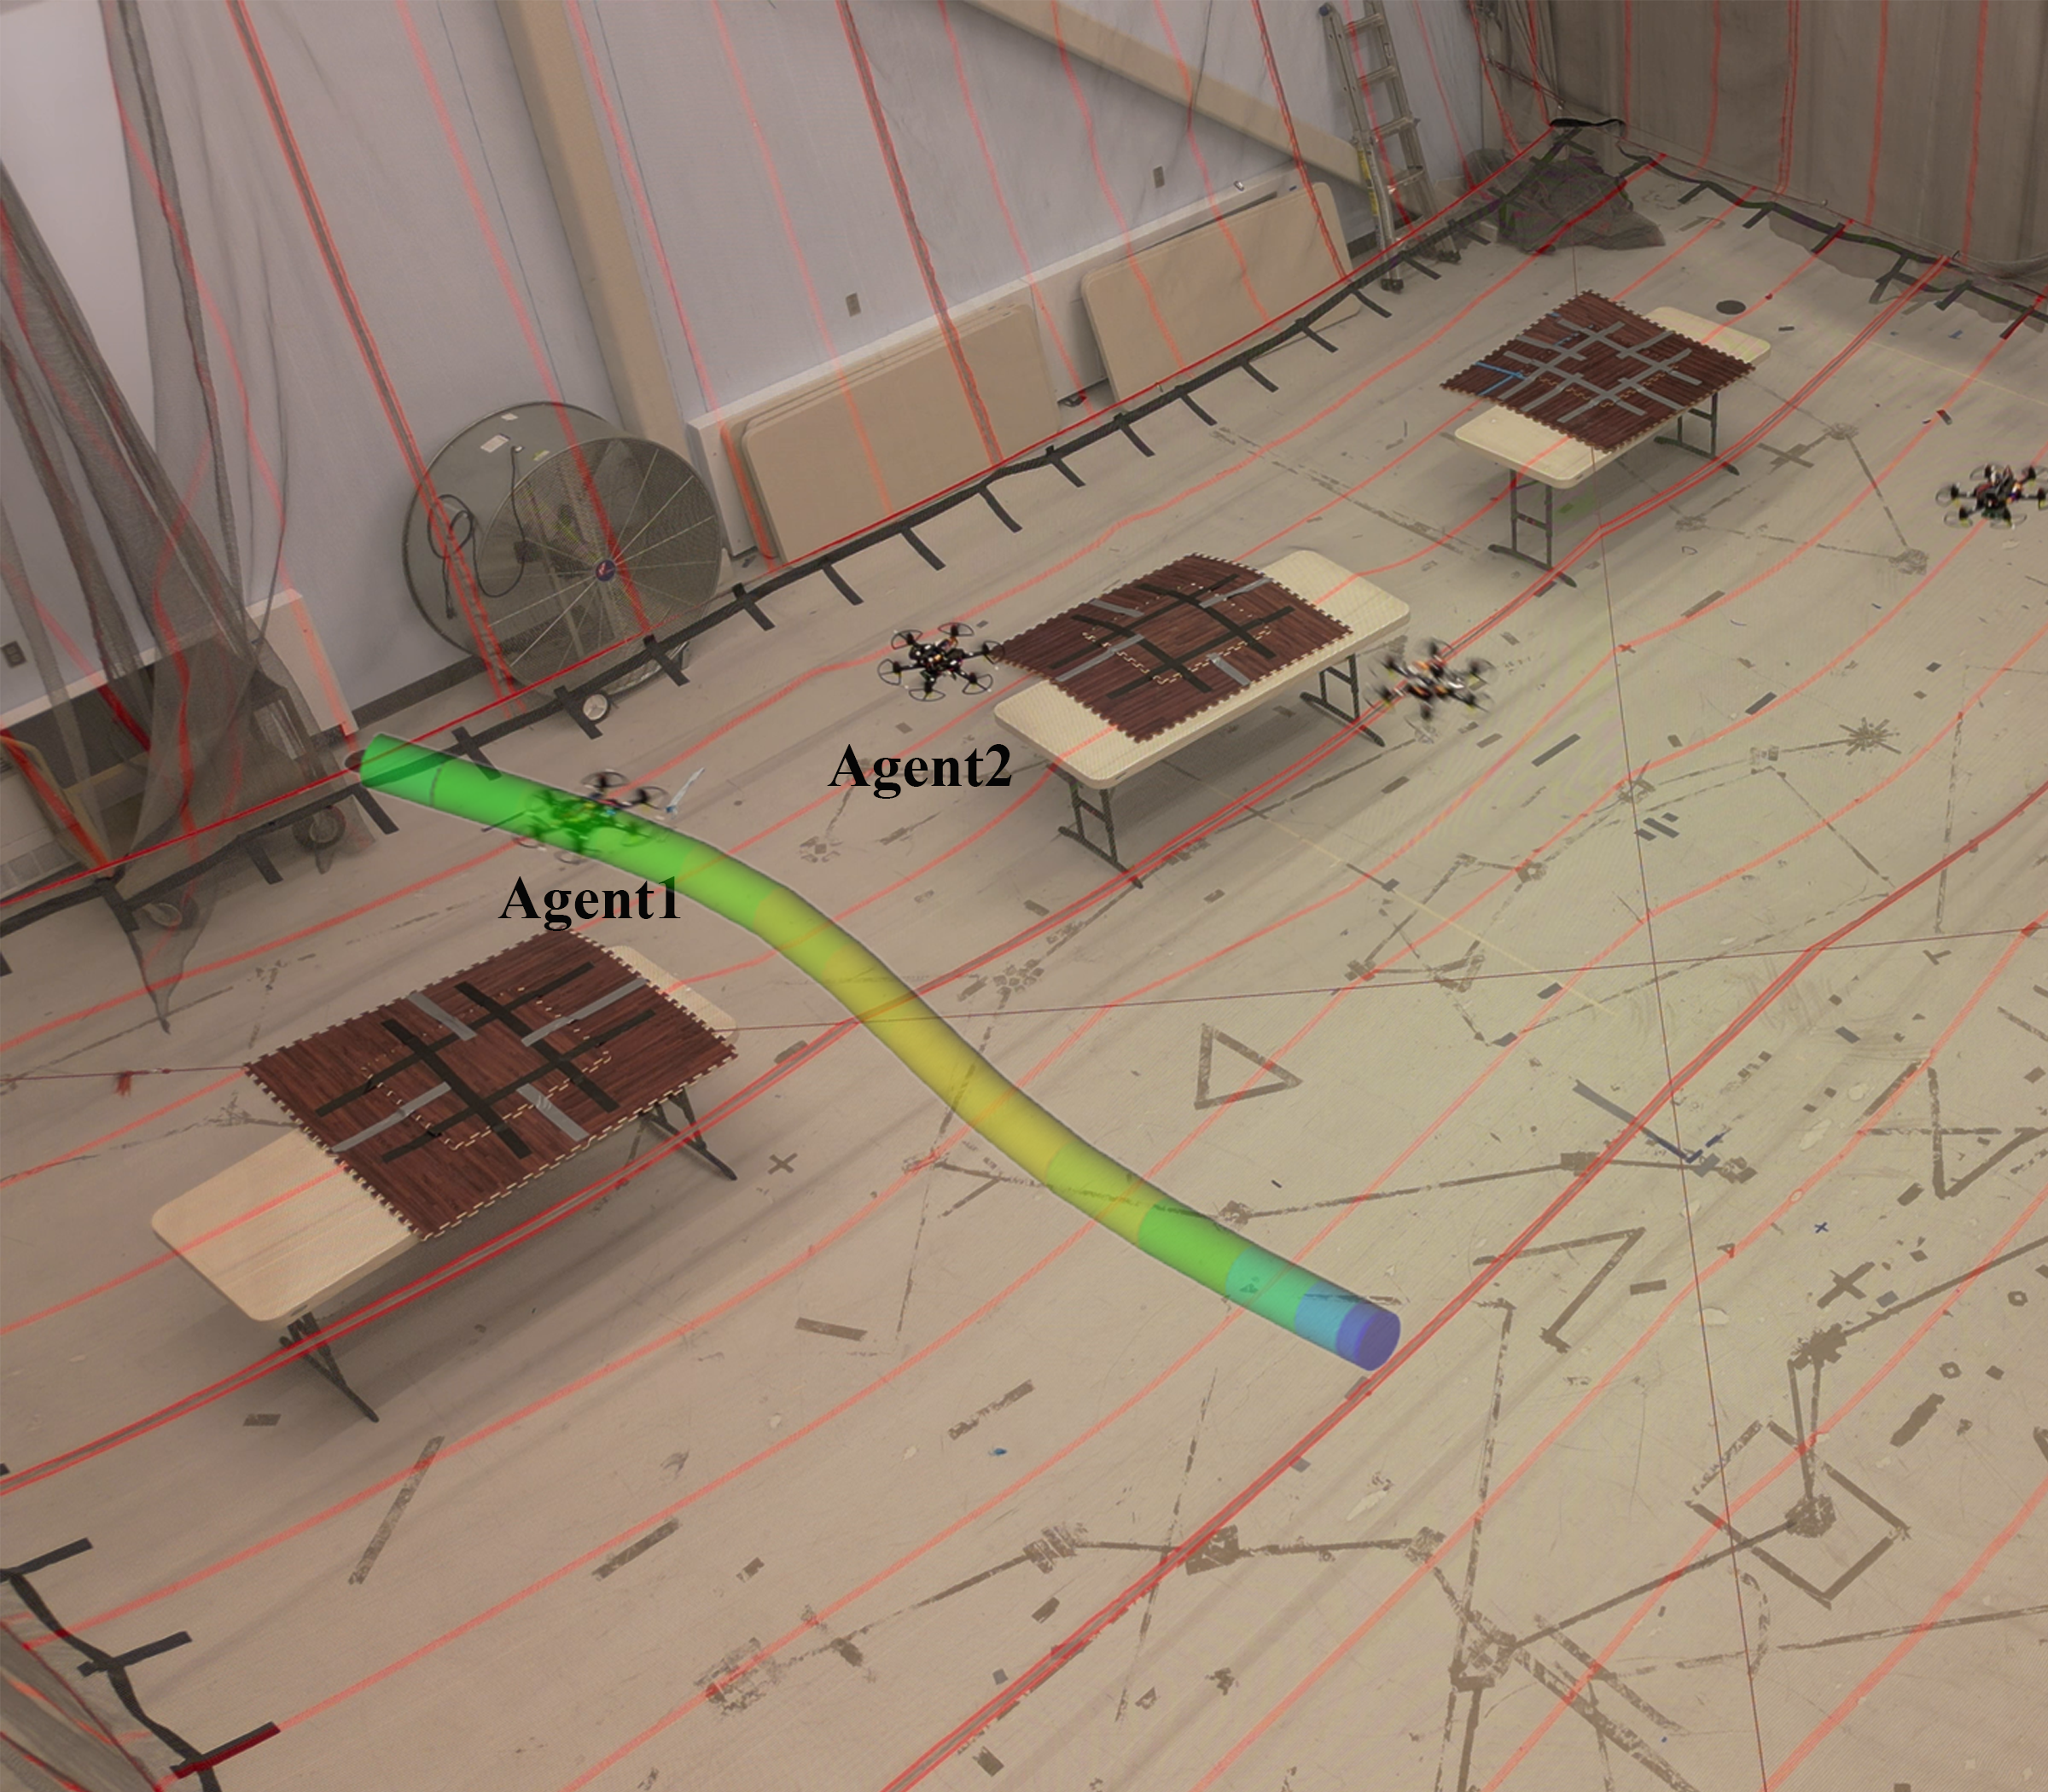
\includegraphics[width=0.3\columnwidth, keepaspectratio]{figures/combined1.png}}
    \subfloat{\includegraphics[width=0.3\columnwidth, keepaspectratio]{figures/rb-DJI-view1.png}}
    \\ {\scriptsize $t=$ \SI{0}{\s}: Agent 1 is following its trajectory} \\[1em]
    \subfloat{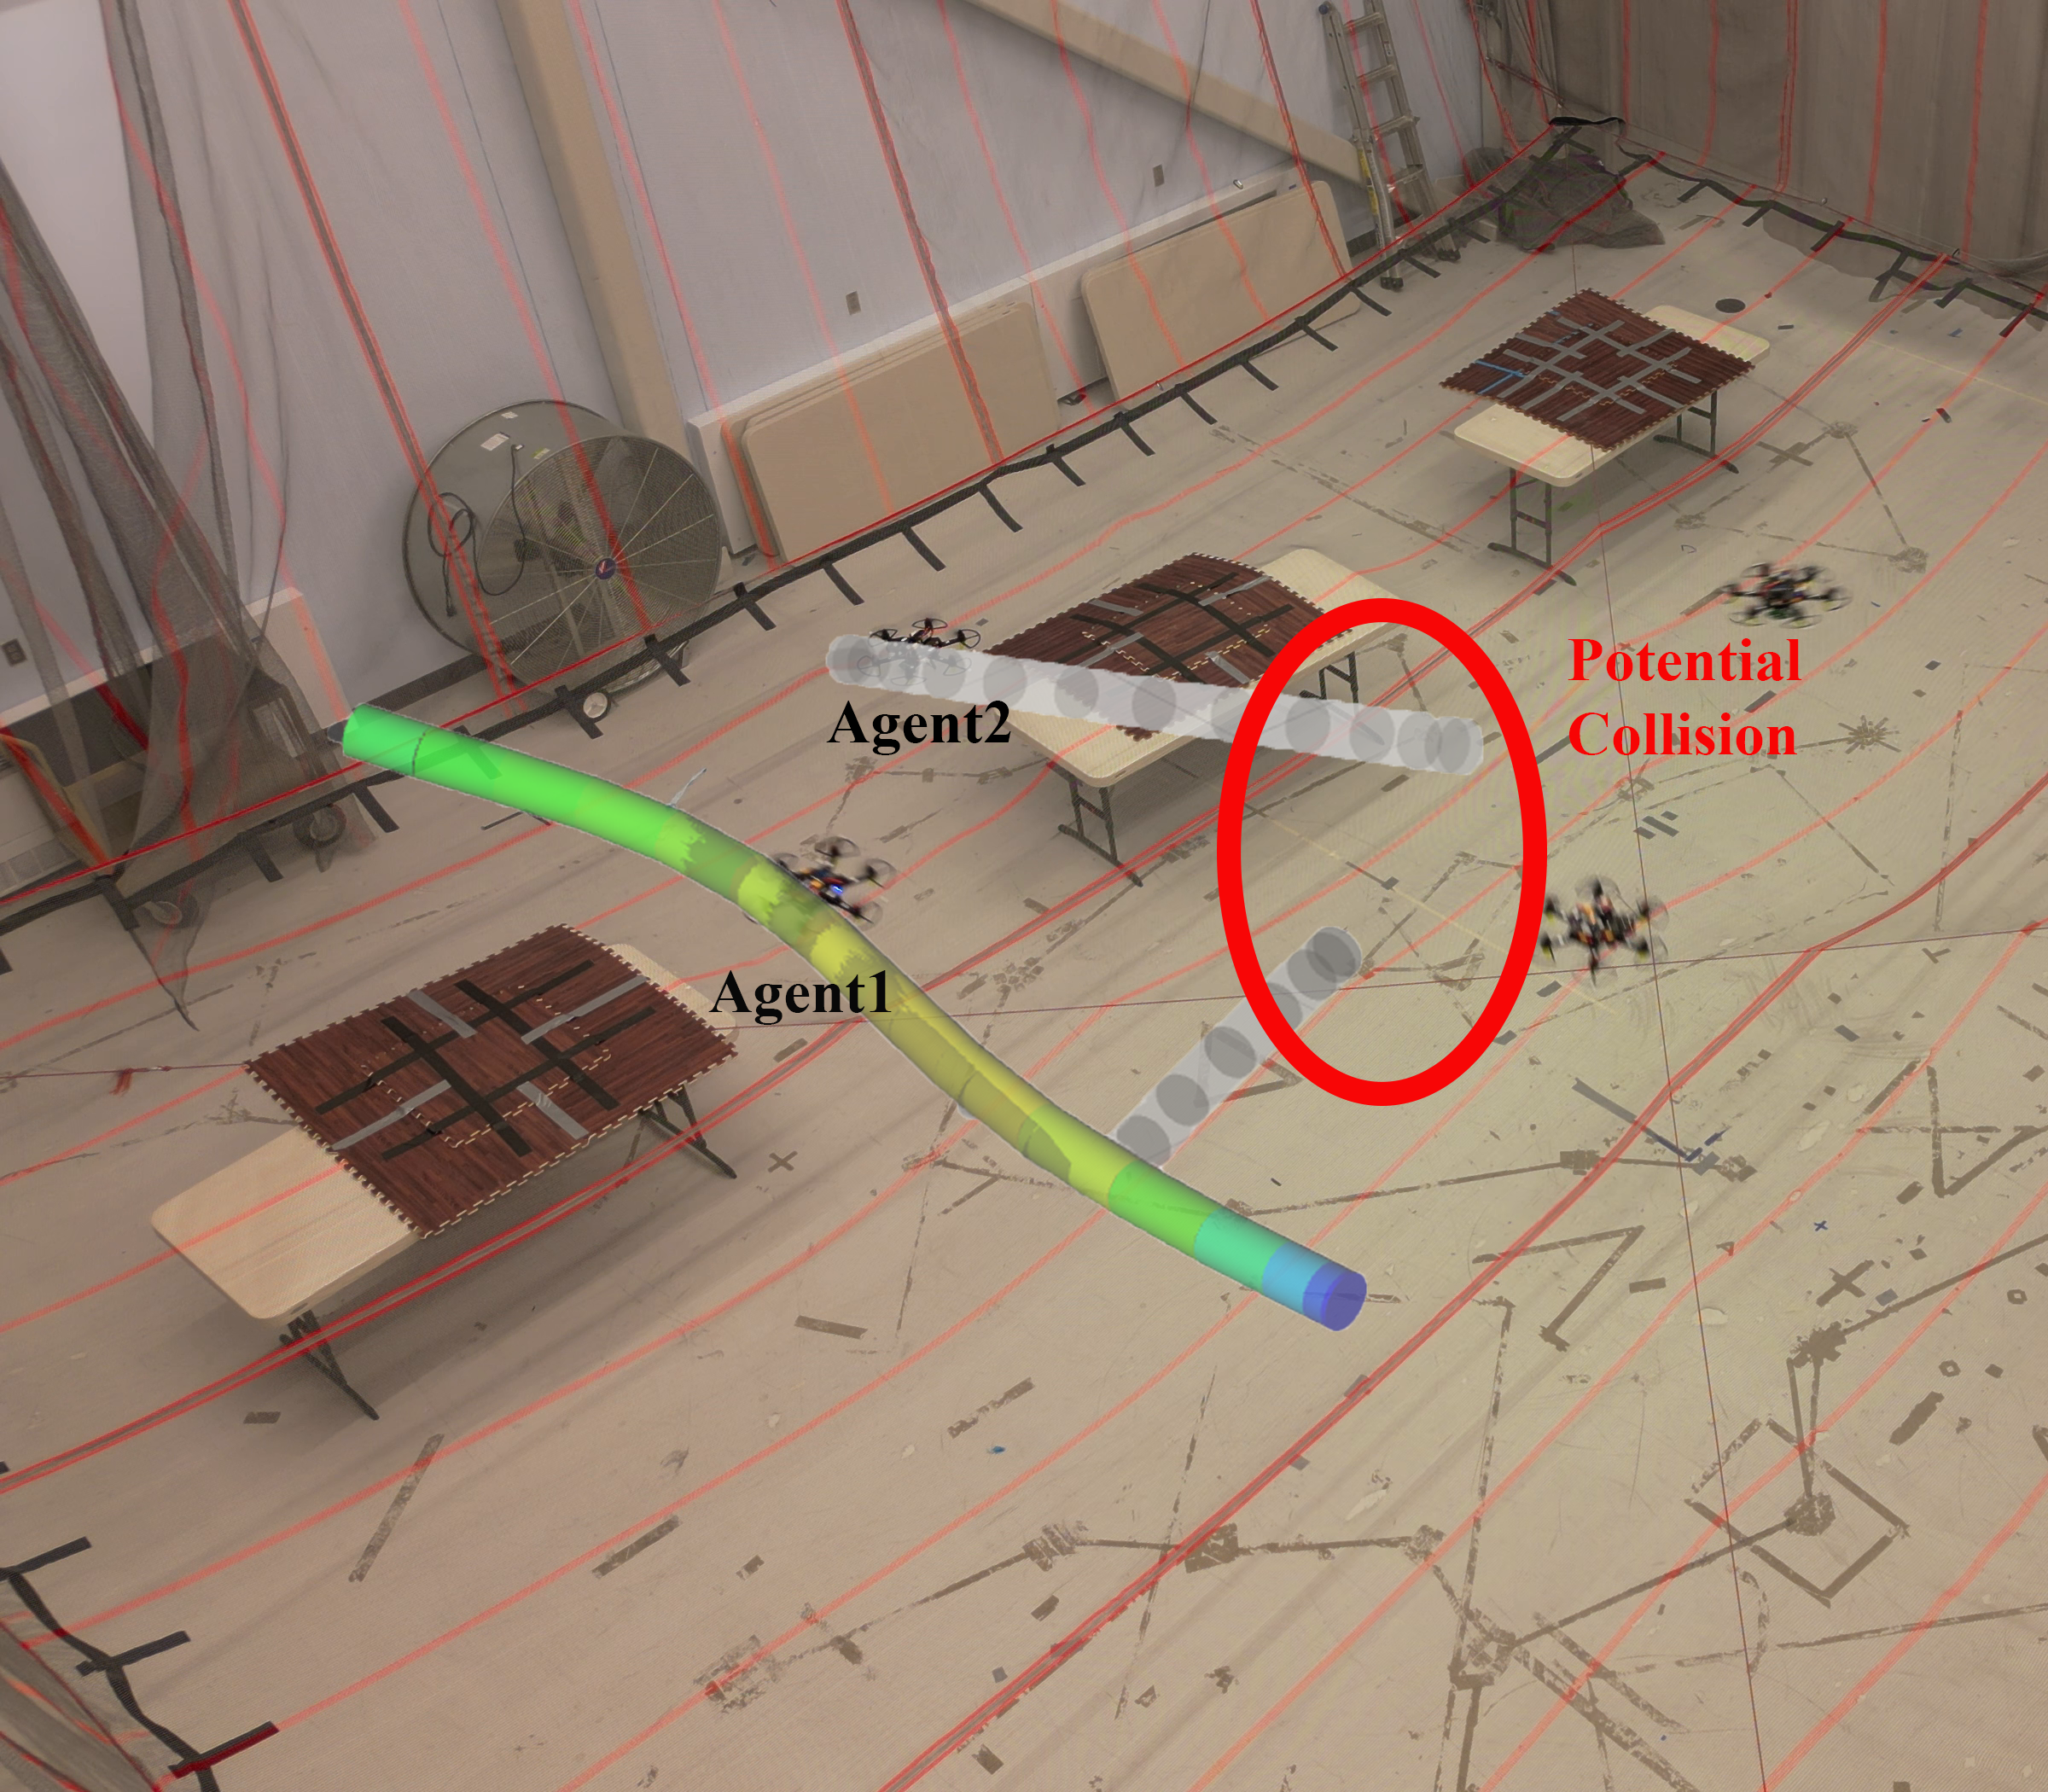
\includegraphics[width=0.3\columnwidth, keepaspectratio]{figures/combined2.png}} 
    \subfloat{\includegraphics[width=0.3\columnwidth, keepaspectratio]{figures/rb-DJI-view2-with-top.png}} 
    \\ {\scriptsize $t=$ \SI{0.15}{\s}: Agent 1 and Agent 2 published their traj\textsubscript{new} only \SI{10}{\ms} apart. Due to communication delays, each agent did not consider the other trajectory, and thus these two trajectories conflict. Note that we have a \SI{1.5}{\m}-tall boundary box, and thus these trajectories are in collision.} \\[1em]
    %\centering
    \subfloat{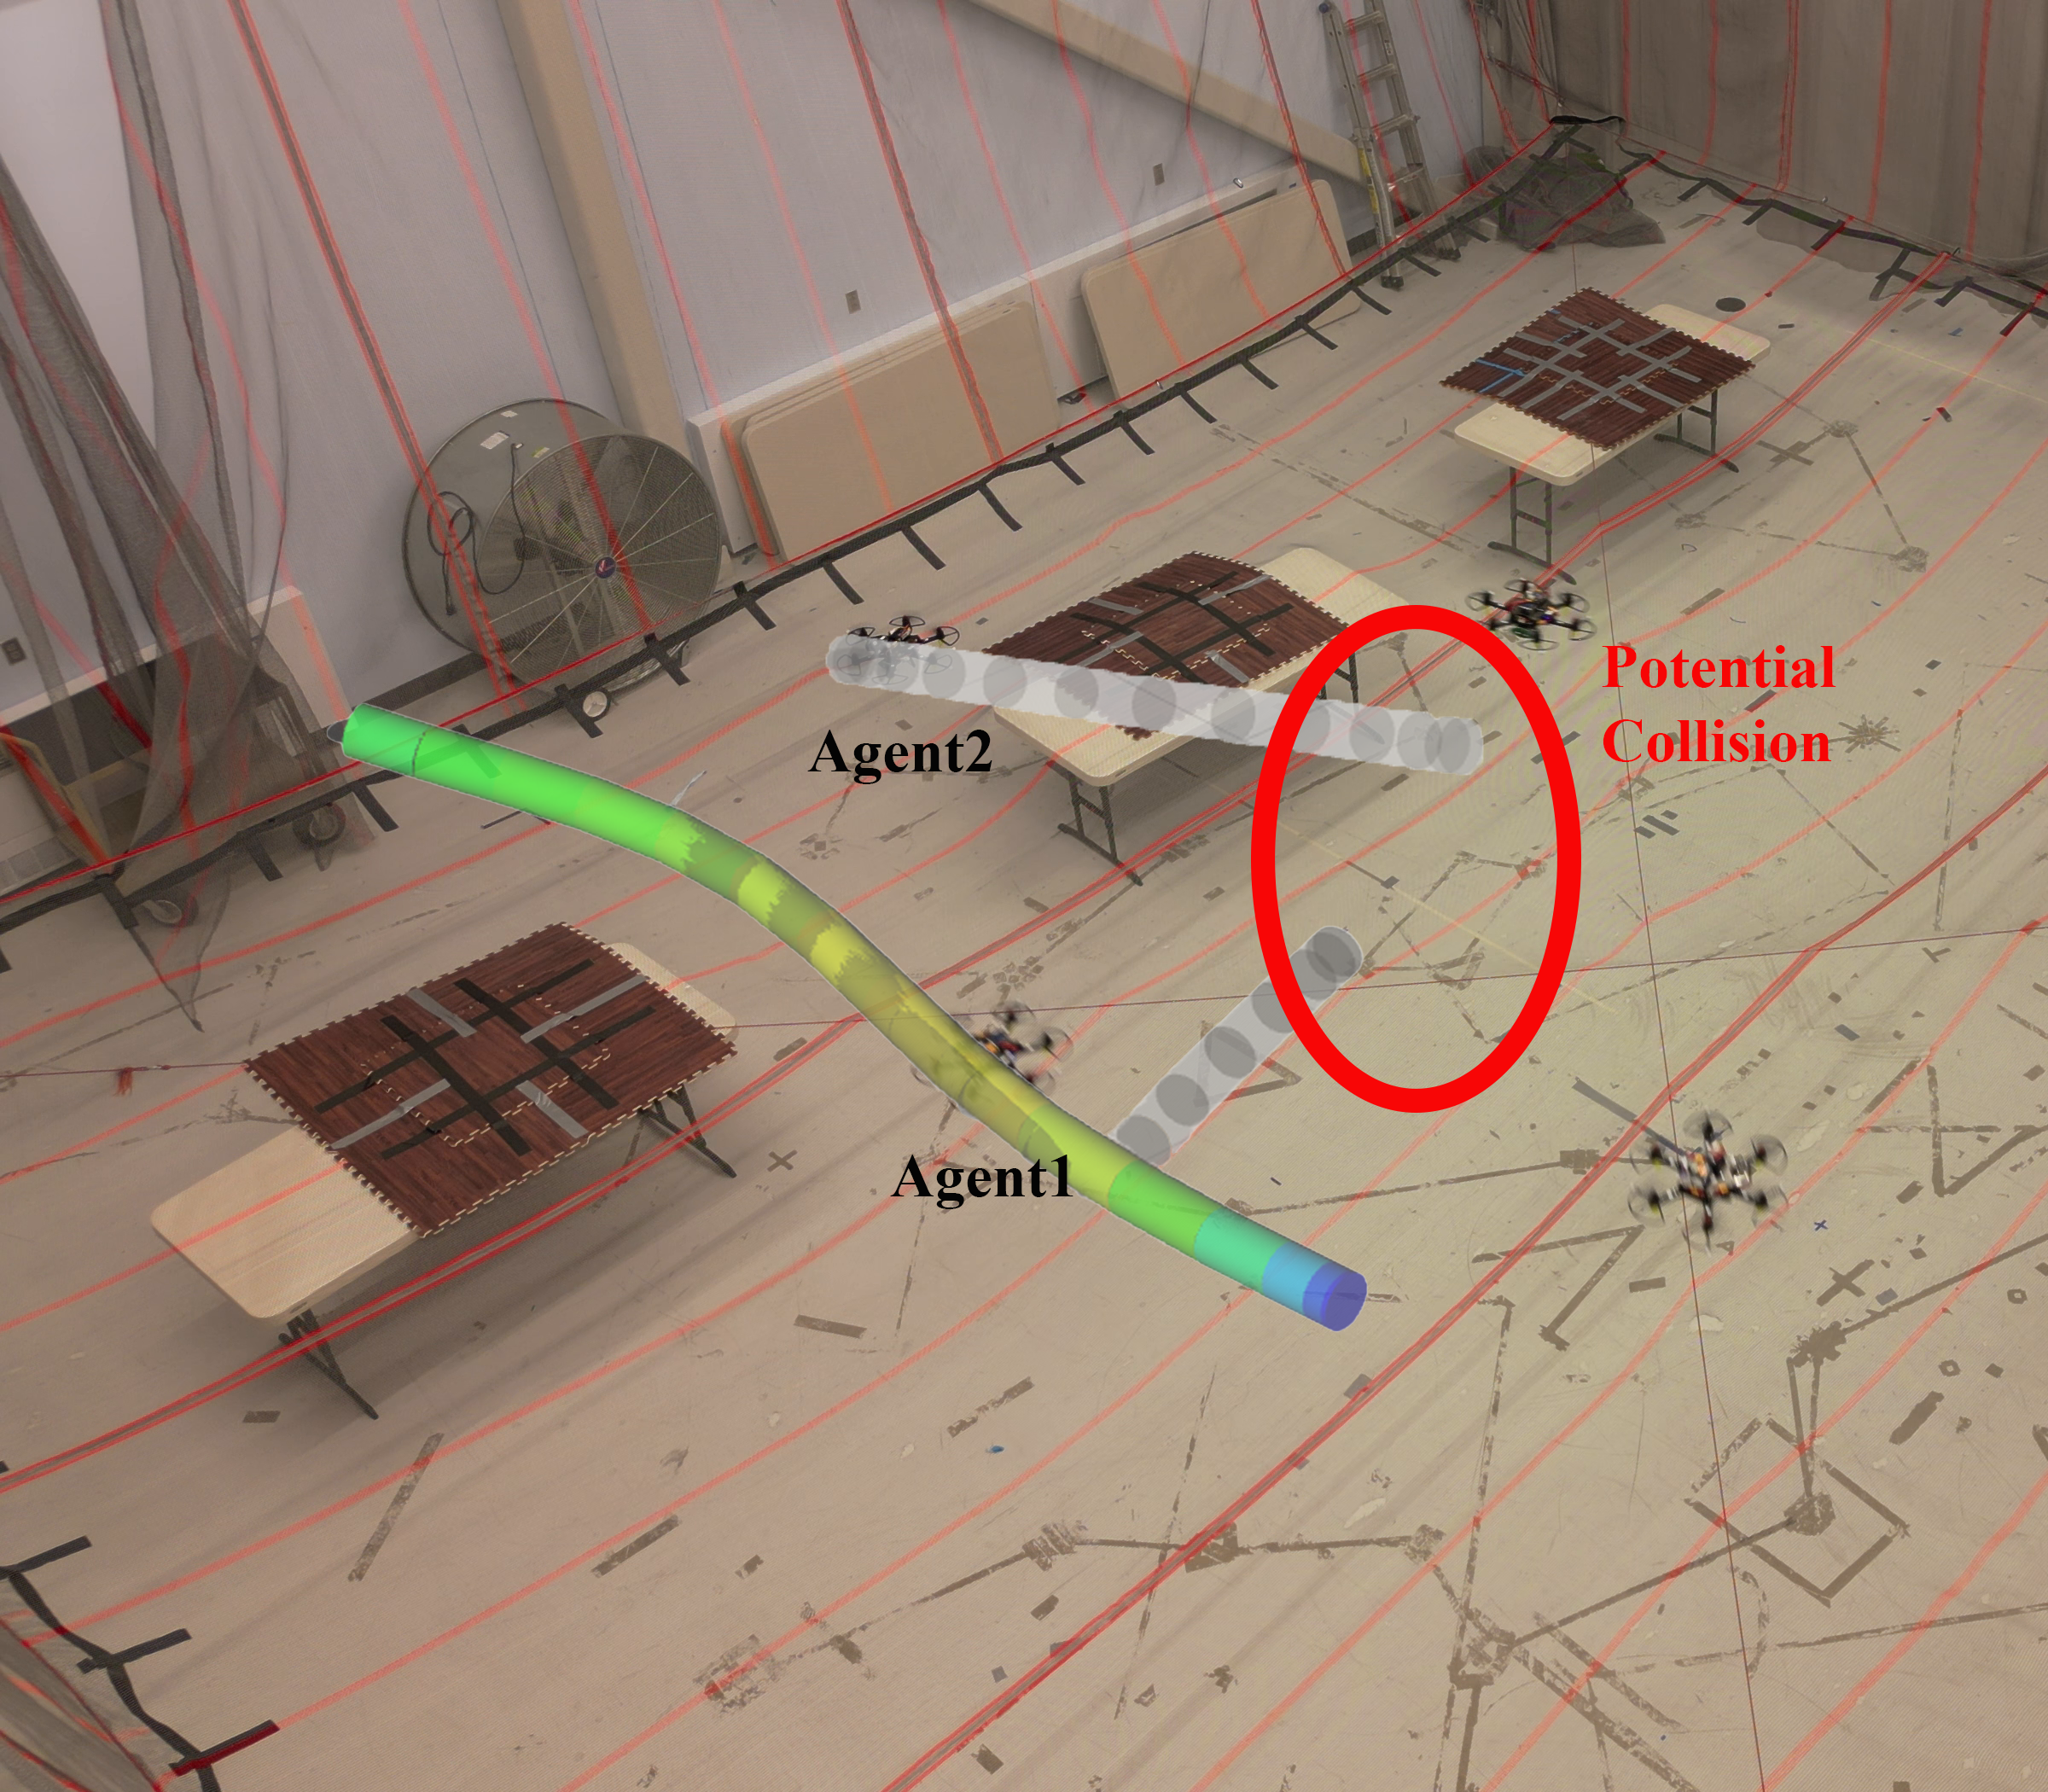
\includegraphics[width=0.3\columnwidth, keepaspectratio]{figures/combined3.png}} 
    \subfloat{\includegraphics[width=0.3\columnwidth, keepaspectratio]{figures/rb-DJI-view3.png}} 
    \\ {\scriptsize $t=$ \SI{1.01}{\s}: During Delay Check both agents detected conflicts and did not commit their trajectory.} \\[1em]
    \subfloat{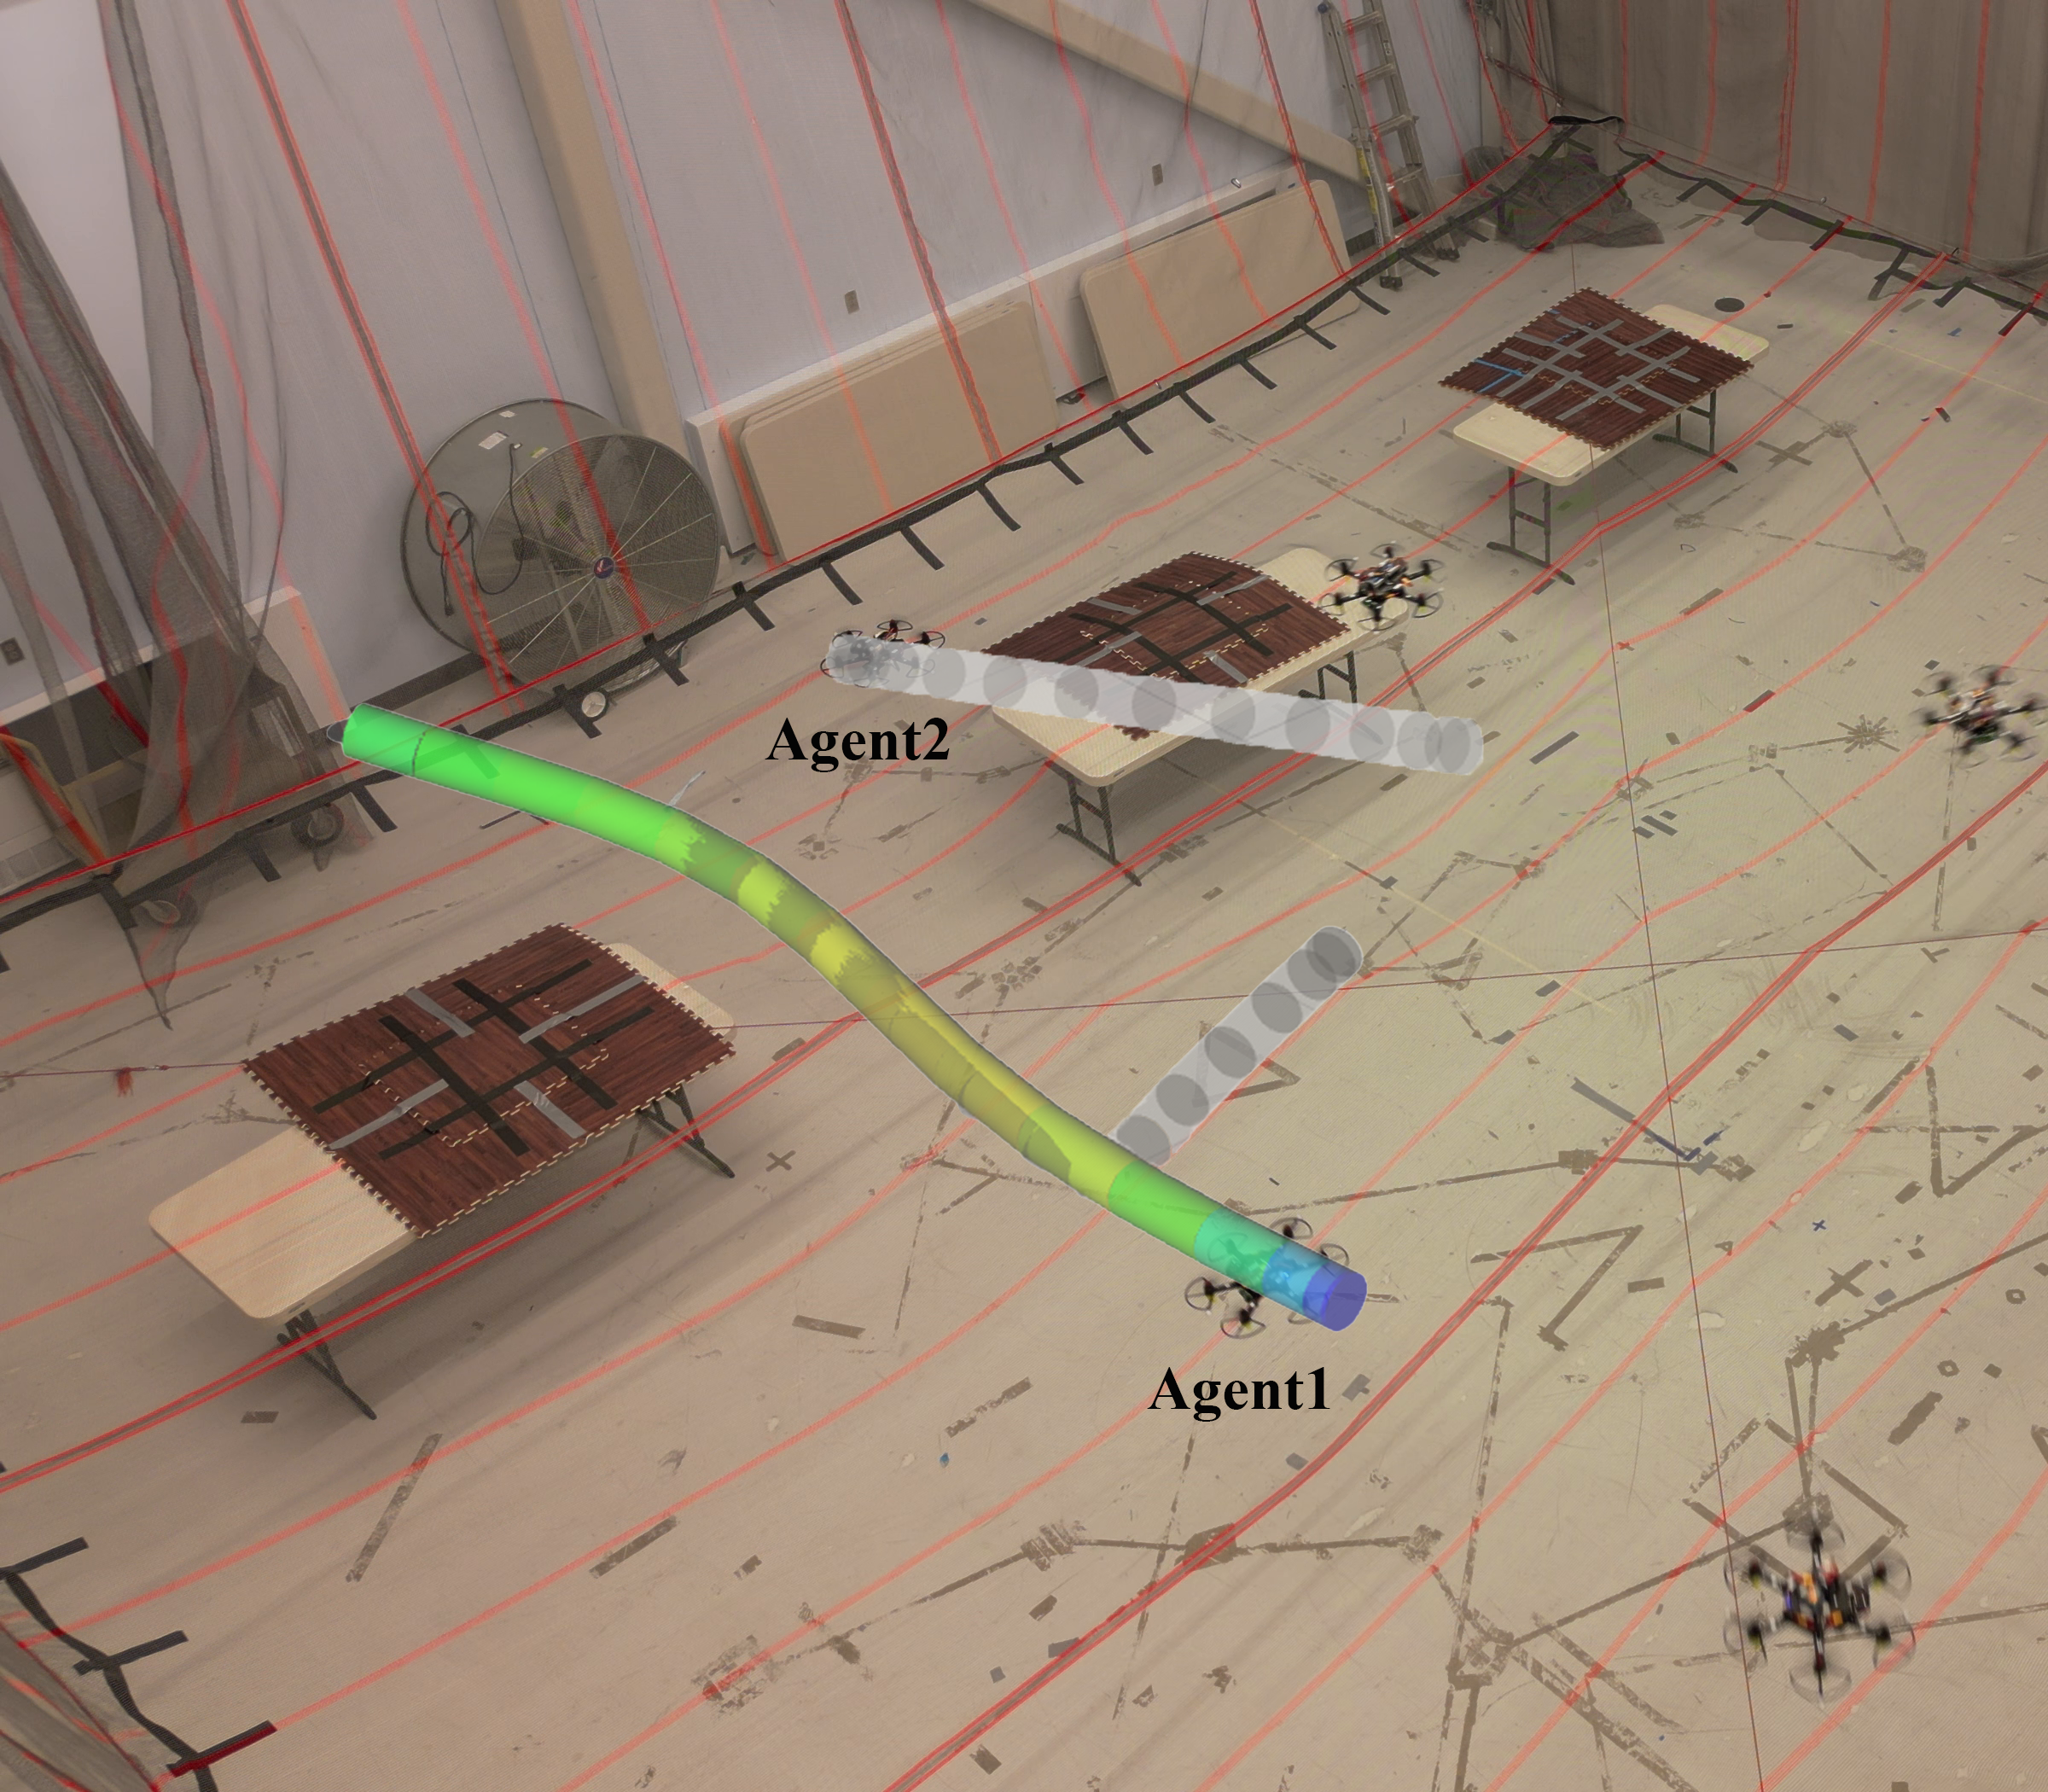
\includegraphics[width=0.3\columnwidth, keepaspectratio]{figures/combined4.png}}
    \subfloat{\includegraphics[width=0.3\columnwidth, keepaspectratio]{figures/rb-DJI-view4.png}}
    \\ {\scriptsize $t=$ \SI{1.97}{\s}: Collision avoided.}
    % \setlength{\belowcaptionskip}{-1em}
    \caption{RMADER successful deconfliction under communication delays}
    \label{fig:rmader_centr}
    \vspace{-1.5em}
\end{figure}

\begin{figure}[!htbp]
    \centering
    \begin{tikzpicture}
    \node (img) {\includegraphics[width=\columnwidth, height=0.22\textheight, keepaspectratio]{figures/6agent_mesh.png}};
    %% circles
    \filldraw[color=black, fill=agent1_color] (-3.2, 1.1) circle (2pt);
    \filldraw[color=black, fill=agent2_color] (-1.2, 2) circle (2pt);
    \filldraw[color=black, fill=agent3_color] (0.05, 2.35) circle (2pt);
    \filldraw[color=black, fill=agent4_color] (0.3, -2.3) circle (2pt);
    \filldraw[color=black, fill=agent5_color] (2.6, 0) circle (2pt);
    \filldraw[color=black, fill=agent6_color] (4, 0.9) circle (2pt);
    %% squares
    \node [rectangle, draw, fill=agent1_color, inner sep=0.7mm] at (1.5, 1.8) {};
    \node [rectangle, draw, fill=agent2_color, inner sep=0.7mm] at (0, 2) {};
    \node [rectangle, draw, fill=agent3_color, inner sep=0.7mm] at (-0.3, 0.85) {};
    \node [rectangle, draw, fill=agent4_color, inner sep=0.7mm] at (0.2, 2.2) {};
    \node [rectangle, draw, fill=agent5_color, inner sep=0.7mm] at (1.1, 0) {};
    \node [rectangle, draw, fill=agent6_color, inner sep=0.7mm] at (-2.1, 0.35) {};
    \end{tikzpicture} 
    % \setlength{\belowcaptionskip}{-1em}
    \caption[6 agents on mesh network]{6 agents on mesh network: Agents move from $\bigcircle$ to \protect\tikz \protect\node [rectangle,draw] at (0,0) {};. Snapshots shown every \SI{500}{ms}.}
    \label{fig:6agent_mesh}
\end{figure}

\begin{table}
\caption{\centering RMADER on Mesh Metwork}
\label{tab:rmader_hw_mesh}
\begin{centering}
% test 2, 17, 19, 24, 30
\renewcommand{\arraystretch}{1.2}
\resizebox{1.0\columnwidth}{!}{
\begin{tabular}{ l c c c c c }
\toprule
 & \textbf{Exp. 11} & \textbf{Exp. 12} & \textbf{Exp. 13} & \textbf{Exp. 14} & \makecell{\textbf{Exp. 15} \\ (fast)}\tabularnewline
\hline 
\hline 
\textbf{Max vel. [m/s]} & 2.7 & 3.0 & 2.9 & 2.8 & 3.0\tabularnewline
\hline 
\textbf{Avg. travel distance [m]} & 46.9 & 48.0 & 49.4 & 66.6 & 60.3 \tabularnewline
\hline
\textbf{Stop time [s]} & 13.7 & 10.6 & 21.4 & 6.2 & 8.8 \tabularnewline
\bottomrule
\end{tabular}}
\par\end{centering}
\end{table}

\subsection{RMADER with Dynamic Obstacles on Mesh Network}
% 4agent2obs/test4, 7
% 6agent2obs/test10, 3, 11
This section illustrates a total of 8 hardware experiments (2 flights for 2 agents with a dynamic obstacle, 2 flights for 4 agents with 2 dynamic obstacles, and 3 flights for 6 agents with 2 dynamic obstacles). 2 and 4-agent experiments lasted \SI{1}{\minute}, and 6 agents exchange their position once. The dynamic constraints are \SI{3.0}{m/s}, \SI{4.0}{m/s^2}, and \SI{5.0}{m/s^3}, but in Experiments 20 and 23, we increased it up to \SI{5.0}{m/s}, \SI{7.0}{m/s^2}, and \SI{10.0}{m/s^3}, and the dynamic obstacles follow randomized trefoil trajectories. 
Table~\ref{tab:rmader_with_obstacles} shows RMADER's performance with obstacles, and Figs~\ref{fig:2agent1obs}, \ref{fig:4agent2obs}, and \ref{fig:rmader_6_agents_with_2_dyn_obs} illustrate 2, 4, and 6 agents with RMADER running onboard successfully carrying out position exchange while avoiding dynamic obstacles.    
Note that due to a hardware issue, one of the 6 agents in Exp. 20-22 was not able to publish its trajectory; however, because it was receiving trajectories from other agents and because of RMADER's decentralized deconfliction mechanism, we observed no collisions. 

\begin{table}
\caption{\centering Hardware experiments with dynamic obstacles}
\label{tab:rmader_with_obstacles}
\begin{centering}
\renewcommand{\arraystretch}{1.2}
\resizebox{1.0\columnwidth}{!}{
\begin{tabular}{ c c | c c c | c c c }
\toprule
& \multicolumn{1}{c}{\makecell{\textbf{2 agents} \\ (1min)}} & \multicolumn{3}{c}{\makecell{\textbf{4 agents} \\ (1min) }} &  \multicolumn{3}{c}{\makecell{\textbf{6 agents} \\ (one time) }}\tabularnewline
 & \makecell{\textbf{Exp. 16} \\ (fast)} & \textbf{Exp. 17} & \textbf{Exp. 18} & \makecell{\textbf{Exp. 19} \\ (fast)} & \textbf{Exp. 20} & \textbf{Exp. 21} & \makecell{\textbf{Exp. 22} \\ (fast)}  \tabularnewline
\hline 
\hline 
\textbf{Max vel. [m/s]} & 4.7 & 3.8 & 3.6 & 5.8 & 3.2 & 3.5 & 5.6 \tabularnewline
\hline 
\makecell{\textbf{Avg. travel} \\ \textbf{distance [m]}} & 106.7 & 114.9 & 109.9 & 114.4 & 24.6 & 23.7 & 22.2 \tabularnewline
\hline
\textbf{Stop time [s]} & 1.60 & 3.51 & 0.90 & 4.91 & 2.42 & 0.76 & 0.76 \tabularnewline
\bottomrule
\end{tabular}
}
\par\end{centering}
\end{table}

\begin{figure}[!htbp]
    \centering
    \begin{tikzpicture}
    \node (img) {\includegraphics[width=\columnwidth, height=0.22\textheight, clip, keepaspectratio]{figures/2agent1obs_test1_post_process.png}};
    %% circles
    \filldraw[color=black, fill=agent1_color] (3.1, 0.2) circle (2pt);
    \filldraw[color=black, fill=agent2_color] (-0.7, -1.7) circle (2pt);
    \filldraw[color=black, fill=obstacle_color] (0.4, 1.0) circle (2pt);
    %% squares
    \node [rectangle, draw, fill=agent1_color, inner sep=0.7mm] at (-3.3, -0.4) {};
    \node [rectangle, draw, fill=agent2_color, inner sep=0.7mm] at (2.0, 0.6) {};
    \node [rectangle, draw, fill=obstacle_color, inner sep=0.7mm] at (1.0, -0.5) {};

    \end{tikzpicture} 
    % \setlength{\belowcaptionskip}{-1em}
    \caption[2 agents with a dynamic obstacle]{2 agents with a dynamic obstacle: agents move from $\bigcircle$ to \protect\tikz \protect\node [rectangle,draw] at (0,0) {};. Snapshots shown every \SI{500}{ms}.}
    \label{fig:2agent1obs}
\end{figure}

\begin{figure}[!htbp]
    \centering
    \begin{tikzpicture}
    \node (img) {\includegraphics[width=\columnwidth, height=0.22\textheight, keepaspectratio]{figures/4agent2obs.png}};
    %% circles
    \filldraw[color=black, fill=agent1_color] (-3.9, -0.1) circle (2pt);
    \filldraw[color=black, fill=agent2_color] (1.9, -0.2) circle (2pt);
    \filldraw[color=black, fill=agent3_color] (-0.7, 0.5) circle (2pt);
    \filldraw[color=black, fill=agent4_color] (3.8, -0.3) circle (2pt);
    \filldraw[color=black, fill=obstacle_color] (-1.65, 0.05) circle (2pt);
    \filldraw[color=black, fill=obstacle_color] (2.6, 0) circle (2pt);
    %% squares
    \node [rectangle, draw, fill=agent1_color, inner sep=0.7mm] at (3.9, 0) {};
    \node [rectangle, draw, fill=agent2_color, inner sep=0.7mm] at (-1.1, -1.4) {};
    \node [rectangle, draw, fill=agent3_color, inner sep=0.7mm] at (1.8, -0.2) {};
    \node [rectangle, draw, fill=agent4_color, inner sep=0.7mm] at (-2.8, 0.6) {};
    \node [rectangle, draw, fill=obstacle_color, inner sep=0.7mm] at (0.65, -0.7) {};
    \node [rectangle, draw, fill=obstacle_color, inner sep=0.7mm] at (2.35, -0.2) {};
    
    \end{tikzpicture} 
    % \setlength{\belowcaptionskip}{-1em}
    \caption[4 agents with 2 dynamic obstacles]{4 agents with 2 dynamic obstacles: agents move from $\bigcircle$ to \protect\tikz \protect\node [rectangle,draw] at (0,0) {};. Snapshots shown every \SI{500}{ms}.}
    \label{fig:4agent2obs}
\end{figure}

\begin{figure}[!htbp]
    \centering
    \subfloat[\scriptsize $t=$ \SIrange{0}{5}{\s}: Agents move from \startbox{} to $\bigcircle$]{
    \begin{tikzpicture}
    \node (img) {\includegraphics[width=\columnwidth, height=0.22\textheight, trim={1.8cm 1cm 3cm 0.7cm}, clip, keepaspectratio]{figures/rmader_hw_six_agents1_legend.pdf}};
    \node [rectangle, draw, fill=agent1_color, inner sep=0.5mm] at (1.2, 2.45) {\tiny start};
    \node [rectangle, draw, fill=agent2_color, inner sep=0.5mm] at (3, -2) {\tiny start};
    \node [rectangle, draw, fill=agent3_color, inner sep=0.5mm] at (0.4, 2.45) {\tiny start};
    \node [rectangle, draw, fill=agent4_color, inner sep=0.5mm] at (1.3, -2.1) {\tiny start};
    \node [rectangle, draw, fill=agent5_color, inner sep=0.5mm] at (-0.5, 2.45) {\tiny start};
    \node [rectangle, draw, fill=agent6_color, inner sep=0.5mm] at (-2, -2.3) {\tiny start};
    \filldraw[color=black, fill=agent1_color] (0.8, 2.4) circle (2pt);
    \filldraw[color=black, fill=agent2_color] (2.1, 0) circle (2pt);
    \filldraw[color=black, fill=agent3_color] (0, 2.4) circle (2pt);
    \filldraw[color=black, fill=agent4_color] (0.5, 0.5) circle (2pt);
    \filldraw[color=black, fill=agent5_color] (-0.7, 1.9) circle (2pt);
    \filldraw[color=black, fill=agent6_color] (-1.3, -0.5) circle (2pt);
    \end{tikzpicture} 
    }    
    \subfloat[\scriptsize $t=$ \SIrange{5}{10}{\s}: Agents move from $\bigcircle$ to \ \rectangle]{
    \begin{tikzpicture}
    \node (img) {\includegraphics[width=\columnwidth, height=0.22\textheight, trim={1.8cm 1cm 3cm 0.7cm}, clip, keepaspectratio]{figures/rmader_hw_six_agents2_legend.pdf}};
    %% circles
    \filldraw[color=black, fill=agent1_color] (1.0, 2.2) circle (2pt);
    \filldraw[color=black, fill=agent2_color] (2.2, 0) circle (2pt);
    \filldraw[color=black, fill=agent3_color] (-0.1, 2.3) circle (2pt);
    \filldraw[color=black, fill=agent4_color] (0.5, 0.5) circle (2pt);
    \filldraw[color=black, fill=agent5_color] (-0.7, 1.9) circle (2pt);
    \filldraw[color=black, fill=agent6_color] (-1.3, -0.5) circle (2pt);
    %% squares
    \node [rectangle, draw, fill=agent1_color, inner sep=0.7mm] at (1.1, 1.8) {};
    \node [rectangle, draw, fill=agent2_color, inner sep=0.7mm] at (-0.8, 2.3) {};
    \node [rectangle, draw, fill=agent3_color, inner sep=0.7mm] at (-0.2, 1.7) {};
    \node [rectangle, draw, fill=agent4_color, inner sep=0.7mm] at (0.1, 2.2) {};
    \node [rectangle, draw, fill=agent5_color, inner sep=0.7mm] at (2.4, -2.2) {};
    \node [rectangle, draw, fill=agent6_color, inner sep=0.7mm] at (0.8, 2.3) {};
    \end{tikzpicture}
    }
    
    \subfloat[\scriptsize $t=$ \SIrange{10}{15}{\s}: Agents move from \rectangle \ to $\triangle$. Agents 2, 5, and 6 reached the goal.]{
    \begin{tikzpicture}
    \node (img) {\includegraphics[width=\columnwidth, height=0.22\textheight, trim={1.8cm 1cm 3cm 0.7cm}, clip, keepaspectratio]{figures/rmader_hw_six_agents3_legend.pdf}};
    %% rectangle
    \node [rectangle, draw, fill=agent1_color, inner sep=0.7mm] at (1.2, 1.9) {};
    \node [rectangle, draw, fill=agent3_color, inner sep=0.7mm] at (-0.2, 1.6) {};
    \node [rectangle, draw, fill=agent4_color, inner sep=0.7mm] at (0.1, 1.9) {};
    %% triangle
    \node [regular polygon, regular polygon sides=3, draw, fill=agent1_color, inner sep=0.4mm] at (0.5, 0.2) {};
    % \node [regular polygon, regular polygon sides=3, draw, fill=agent2_color, inner sep=0.4mm] at (0.5, 0.2) {};
    \node [regular polygon, regular polygon sides=3, draw, fill=agent3_color, inner sep=0.4mm] at (-0.1, -0.2) {};
    \node [regular polygon, regular polygon sides=3, draw, fill=agent4_color, inner sep=0.4mm] at (-0.1, 2.2) {};
    % \node [regular polygon, regular polygon sides=3, draw, fill=agent5_color, inner sep=0.4mm] at (0.5, 0.2) {};
    % \node [regular polygon, regular polygon sides=3, draw, fill=agent6_color, inner sep=0.4mm] at (0.5, 0.2) {};
    %% goal
    \node [rectangle, draw, fill=agent2_color, inner sep=0.5mm] at (-1.0, 2.3) {\tiny goal};
    \node [rectangle, draw, fill=agent5_color, inner sep=0.5mm] at (2.5, -2.2) {\tiny goal};
    \node [rectangle, draw, fill=agent6_color, inner sep=0.5mm] at (1.0, 2.3) {\tiny goal};
    \end{tikzpicture}
    }
    \subfloat[\scriptsize $t=$ \SIrange{15}{20}{\s}: Agents move from $\triangle$ to \goalbox{}]{
    \begin{tikzpicture}
    \node (img) {\includegraphics[width=\columnwidth, height=0.22\textheight, trim={1.8cm 1cm 3cm 0.7cm}, clip, keepaspectratio]{figures/rmader_hw_six_agents4_legend.pdf}};
    \node [regular polygon, regular polygon sides=3, draw, fill=agent1_color, inner sep=0.4mm] at (0.5, 0.2) {};
    \node [regular polygon, regular polygon sides=3, draw, fill=agent3_color, inner sep=0.4mm] at (-0.1, -0.2) {};
    %% goal
    \node [rectangle, draw, fill=agent1_color, inner sep=0.5mm] at (-2.7, -2.1) {\tiny goal};
    \node [rectangle, draw, fill=agent2_color, inner sep=0.5mm] at (-1.0, 2.3) {\tiny goal};
    \node [rectangle, draw, fill=agent3_color, inner sep=0.5mm] at (-0.2, -2.1) {\tiny goal};
    \node [rectangle, draw, fill=agent4_color, inner sep=0.5mm] at (0.3, 2.3) {\tiny goal};
    \node [rectangle, draw, fill=agent5_color, inner sep=0.5mm] at (2.5, -2.2) {\tiny goal};
    \node [rectangle, draw, fill=agent6_color, inner sep=0.5mm] at (1.0, 2.3) {\tiny goal};
    \end{tikzpicture}
    }
    \caption[6 agents with 2 dynamic obstacles]{\centering 6 agent hardware experiments with 2 dynamic obstacles. Snapshots shown every \SI{500}{ms}}
    \label{fig:rmader_6_agents_with_2_dyn_obs}
\end{figure}

\cleardoublepage
\newpage